\documentclass{article}
\usepackage[]{graphicx}
\graphicspath{ {./images/} }
\usepackage[]{color}
%\usepackage{hyperref}

\usepackage[colorlinks=true,linkcolor=blue]{hyperref}

\usepackage{listings}

\definecolor{dkgreen}{rgb}{0,0.6,0}
\definecolor{gray}{rgb}{0.5,0.5,0.5}
\definecolor{mauve}{rgb}{0.58,0,0.82}

\lstset{frame=tb,
  language=bash,
  aboveskip=3mm,
  belowskip=3mm,
  showstringspaces=false,
  columns=flexible,
  basicstyle={\small\ttfamily},
  numbers=none,
  numberstyle=\tiny\color{gray},
  keywordstyle=\color{blue},
  commentstyle=\color{dkgreen},
  stringstyle=\color{red},
  breaklines=true,
  breakatwhitespace=true,
  tabsize=3
}

\usepackage{enumitem}% http://ctan.org/pkg/enumitem

% maxwidth is the original width if it is less than linewidth
% otherwise use linewidth (to make sure the graphics do not exceed the margin)
\makeatletter
\def\maxwidth{ %
  \ifdim\Gin@nat@width>\linewidth
    \linewidth
  \else
    \Gin@nat@width
  \fi
}
\makeatother

\definecolor{fgcolor}{rgb}{0.345, 0.345, 0.345}
\newcommand{\hlnum}[1]{\textcolor[rgb]{0.686,0.059,0.569}{#1}}%
\newcommand{\hlstr}[1]{\textcolor[rgb]{0.192,0.494,0.8}{#1}}%
\newcommand{\hlcom}[1]{\textcolor[rgb]{0.678,0.584,0.686}{\textit{#1}}}%
\newcommand{\hlopt}[1]{\textcolor[rgb]{0,0,0}{#1}}%
\newcommand{\hlstd}[1]{\textcolor[rgb]{0.345,0.345,0.345}{#1}}%
\newcommand{\hlkwa}[1]{\textcolor[rgb]{0.161,0.373,0.58}{\textbf{#1}}}%
\newcommand{\hlkwb}[1]{\textcolor[rgb]{0.69,0.353,0.396}{#1}}%
\newcommand{\hlkwc}[1]{\textcolor[rgb]{0.333,0.667,0.333}{#1}}%
\newcommand{\hlkwd}[1]{\textcolor[rgb]{0.737,0.353,0.396}{\textbf{#1}}}%
\let\hlipl\hlkwb

\usepackage{framed}
\makeatletter
\newenvironment{kframe}{%
 \def\at@end@of@kframe{}%
 \ifinner\ifhmode%
  \def\at@end@of@kframe{\end{minipage}}%
  \begin{minipage}{\columnwidth}%
 \fi\fi%
 \def\FrameCommand##1{\hskip\@totalleftmargin \hskip-\fboxsep
 \colorbox{shadecolor}{##1}\hskip-\fboxsep
     % There is no \\@totalrightmargin, so:
     \hskip-\linewidth \hskip-\@totalleftmargin \hskip\columnwidth}%
 \MakeFramed {\advance\hsize-\width
   \@totalleftmargin\z@ \linewidth\hsize
   \@setminipage}}%
 {\par\unskip\endMakeFramed%
 \at@end@of@kframe}
\makeatother

\definecolor{shadecolor}{rgb}{.97, .97, .97}
\definecolor{messagecolor}{rgb}{0, 0, 0}
\definecolor{warningcolor}{rgb}{1, 0, 1}
\definecolor{errorcolor}{rgb}{1, 0, 0}
\newenvironment{knitrout}{}{} % an empty environment to be redefined in TeX

\usepackage{alltt}

\title{Getting Started with Raspberry Pi}
\IfFileExists{upquote.sty}{\usepackage{upquote}}{}


\author{Kyle McCarty and Marc Los Huertos\footnote{Acknowledgments: Summer research students, Anna Burns and Alision Joseph contributed to these documents.}}
\title{Getting Started with Raspberry Pi}

\begin{document}

\maketitle

\newpage

\tableofcontents

\newpage

\section{Introduction}

\subsection{What is a Raspberry Pi?}

The Raspberry Pi is an tiny computer, that includes a microprocessor, a bit of memory, a slot for an SD card, input/output (I/O) ports, e.g. HDMI, USB, headphone, camera, and some general purpose input/output (GPIO) pins for various types of electrical connectors.

\subsection{Why use the Raspberry Pi?}

Generally, Raspberry Pis draw considerably less power than regular computers, are a lot smaller, and are relatively cost-effective. In addition, the GPIO pins allow for connecting and controlling various types of electrical components, such as LEDs and sensors. Raspberry Pis are very flexible devices. They can be used for personal computers, home survaillance systems, weather stations, adblockers for your home network, retro gaming machines, as an AI assistant, and so much more! In this class, we'll be using it as an environmental monitoring device.

\section{Unpacking and Connecting the Pi}

\subsection{Packaging List}

\subsubsection{``Vilros RP Zero W Basics Kit''}

\begin{enumerate}[noitemsep]
  \item Raspberry Pi Zero W board
  \item Vilros Case, with 3 covers
  \item 2.5A power supply
  \item Heatsink
  \item HDMI to mini-HDMI adapter
  \item USB to micro-USB adapter
  \item Header pin diagram
  \item Camera module cable (not used)
\end{enumerate}

\subsubsection{Other items}

\begin{enumerate}[noitemsep]
  \item SD card
  \item SD card to USB adapter
  \item USB multiport adapter
  \item Breadboard
  \item Wires
  \item Line level converter (LLC)
  \item MCP3008
  \item various MQ-sensors

\end{enumerate}

\subsection{Install Raspberry Pi OS on SD card}

\begin{enumerate}
  \item Download Raspberry Pi Imager for your main computer's operating system (OS) at \url{https://www.raspberrypi.org/downloads/}
  \item Install Raspberry Pi Imager
  \item Connect the Pi's SD card to your main computer.
  
\begin{figure}
\centering
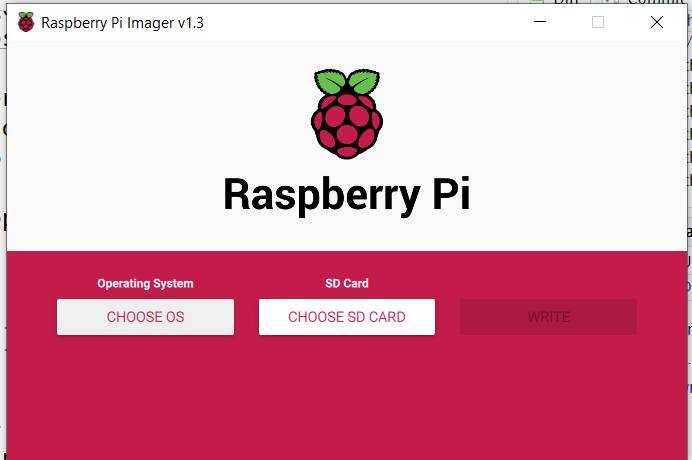
\includegraphics[width=1.00\textwidth]{1_Pi_Imager}
%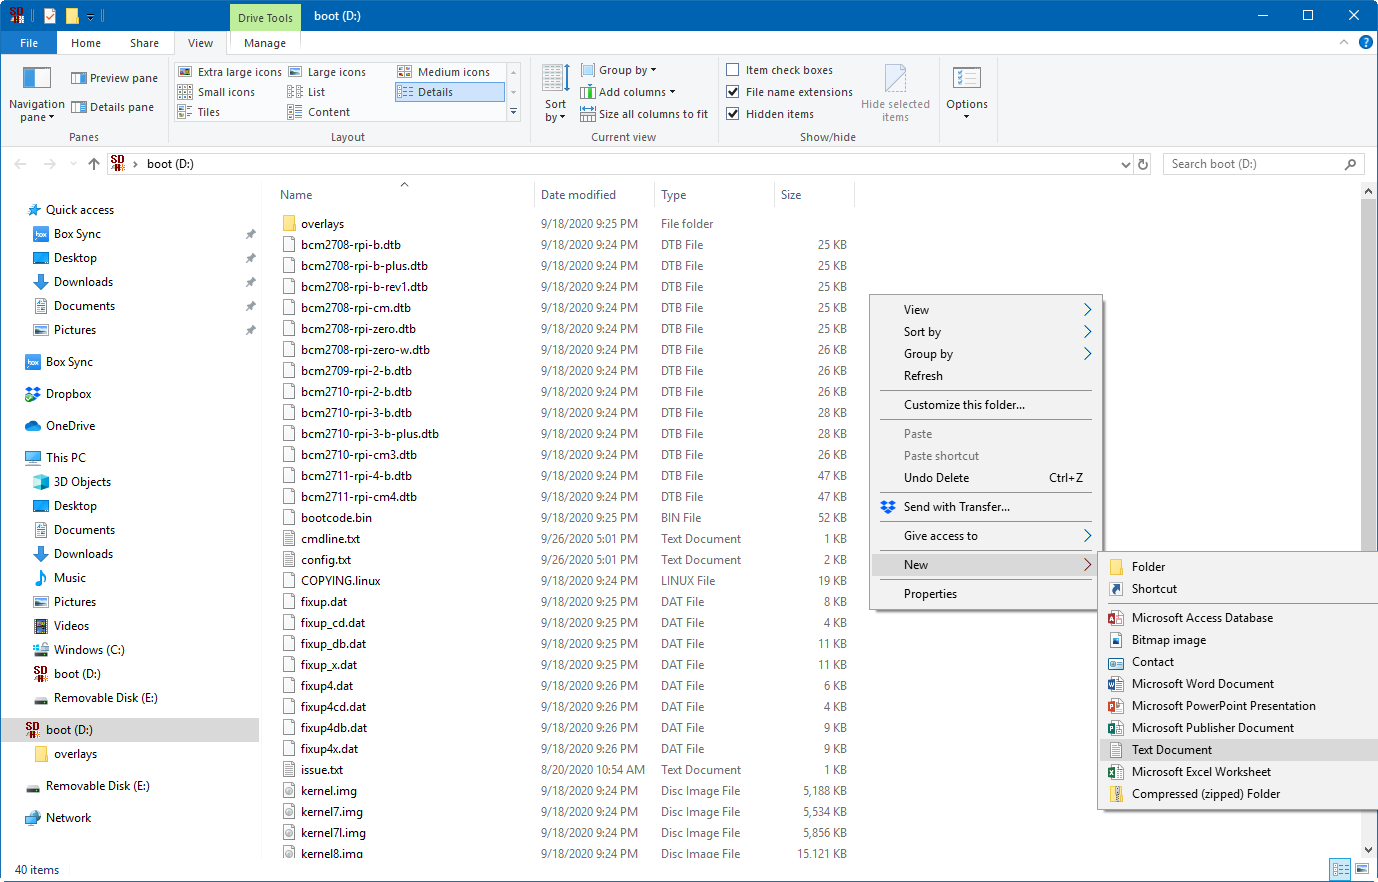
\includegraphics[width=1.00\textwidth]{sdbootnew}
\caption{Raspberry Pi Image Software. Use the program to select Raspberry Pi OS (Operating System) 32-bit. Then select the SD card location. Finally, click on ``Write''.}
\label{fig:pi_imager}
\end{figure}

  \item Use Raspberry Pi Imager to install/write Raspberry Pi OS to SD card (Figure~\label{fig:pi_imager}).
  \item Alternatively, manually copy Raspberry Pi OS and NOOBS to SD card, using the link above.
\end{enumerate}

\subsection{Create Secure Shell Connectivity Files} \label{networkssh}

\begin{enumerate}
  \item Add a ``ssh'' file to your SD card.\footnote{What is SSH protocol? SSH, also referred to as Secure Shell, is a method for secure remote login from one computer to another. It provides several alternative options for strong authentication, and it protects the communications security and integrity with strong encryption.} When the Raspberry Pi boots up, it will look for a file named \textbf{``ssh''} to determine if one can remotely login to the Pi. If the file is there, then remote login is enabled. If the file is not present, then remote login is disabled. 
  \begin{itemize}
  \item Do this by creating an empty text file named \textbf{``ssh''}. Doing this on PCs is really easy -- but as on Apple computers it frustratingly complex. 
  
\noindent\textbf{For Mac Users:} 

\begin{itemize}
  \item Find and start the TextEdit application (Figure~\ref{fig:Mac1}).
  
\begin{figure}[!h]
\centering
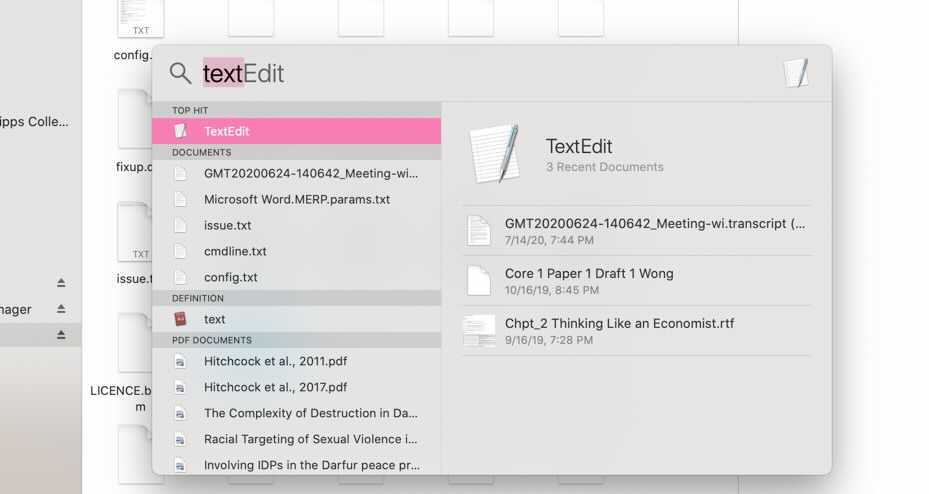
\includegraphics[width=0.9\textwidth]{1_MACtext_1}
\caption{Finding the TextEdit application}
\label{fig:Mac1}
\end{figure}

  \item Save file (Figure~\ref{fig:Mac2}).

\begin{figure}[h]
\centering
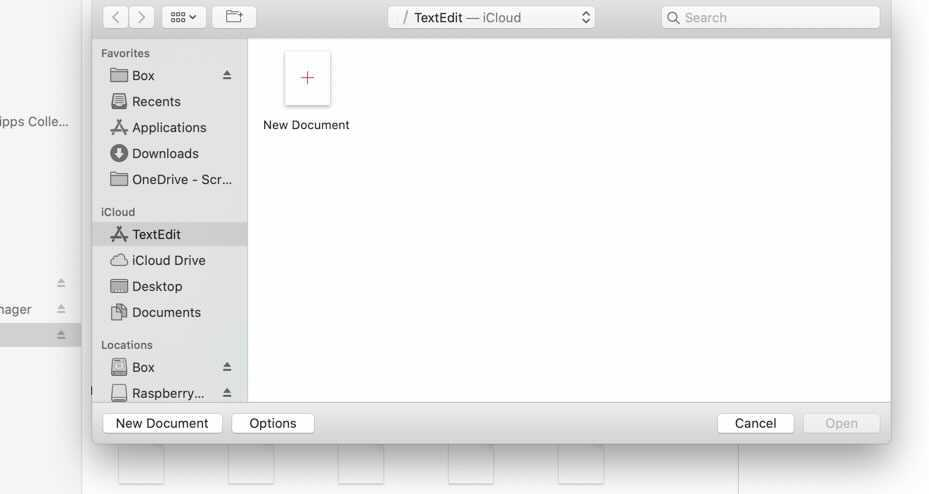
\includegraphics[width=0.9\textwidth]{1_MACtext_2}
\caption{Save file with out richtext formatting.}
\label{fig:Mac2}
\end{figure}

  \item Open a new document (Figure~\ref{fig:Mac3}).

\begin{figure}[h]
\centering
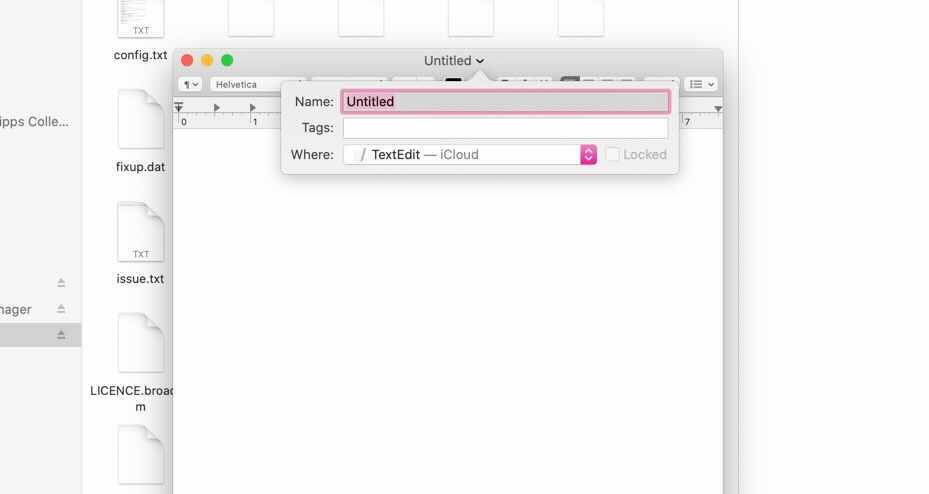
\includegraphics[width=1.0\textwidth]{1_MACtext_3}
\caption{Save empty file}
\label{fig:Mac3}
\end{figure}
  \item Save file without richtext (Figure~\ref{fig:Mac4}).

\begin{figure}[h]
\centering
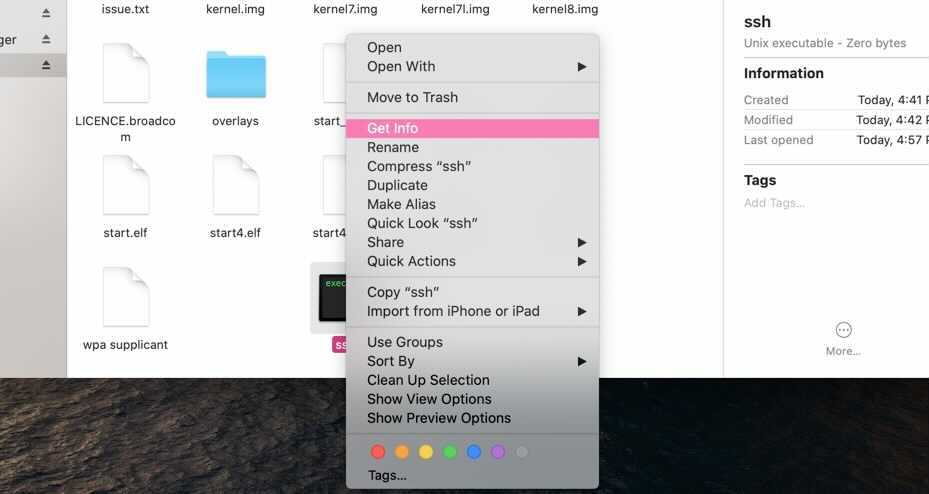
\includegraphics[width=1.0\textwidth]{1_MACtext_4}
\caption{Get information on the file}
\label{fig:Mac4}
\end{figure}

  \item Remove extension. (Figure~\ref{fig:Mac5}).

\begin{figure}[h]
\centering
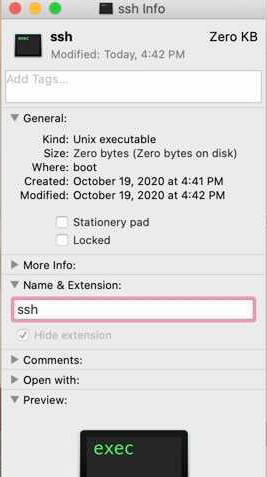
\includegraphics[width=0.50\textwidth]{1_MACtext_5}
\caption{Remove file name extension.}
\label{fig:Mac5}
\end{figure}

\end{itemize}

\noindent \textbf{For PC Users:} 

  \item Start a text editor and create an empty file named ``ssh''. Make sure the file you create has no file extension. You will have to ``Save As'' with your text editor to ensure the file is saved the correct way; meaning the file shouldn't end in ``.txt'', ``.doc'', etc. Sometimes there is the option from a dropdown to change the file extension.
  
\item Copy ``ssh'' file to the SD card. 
\begin{figure}
  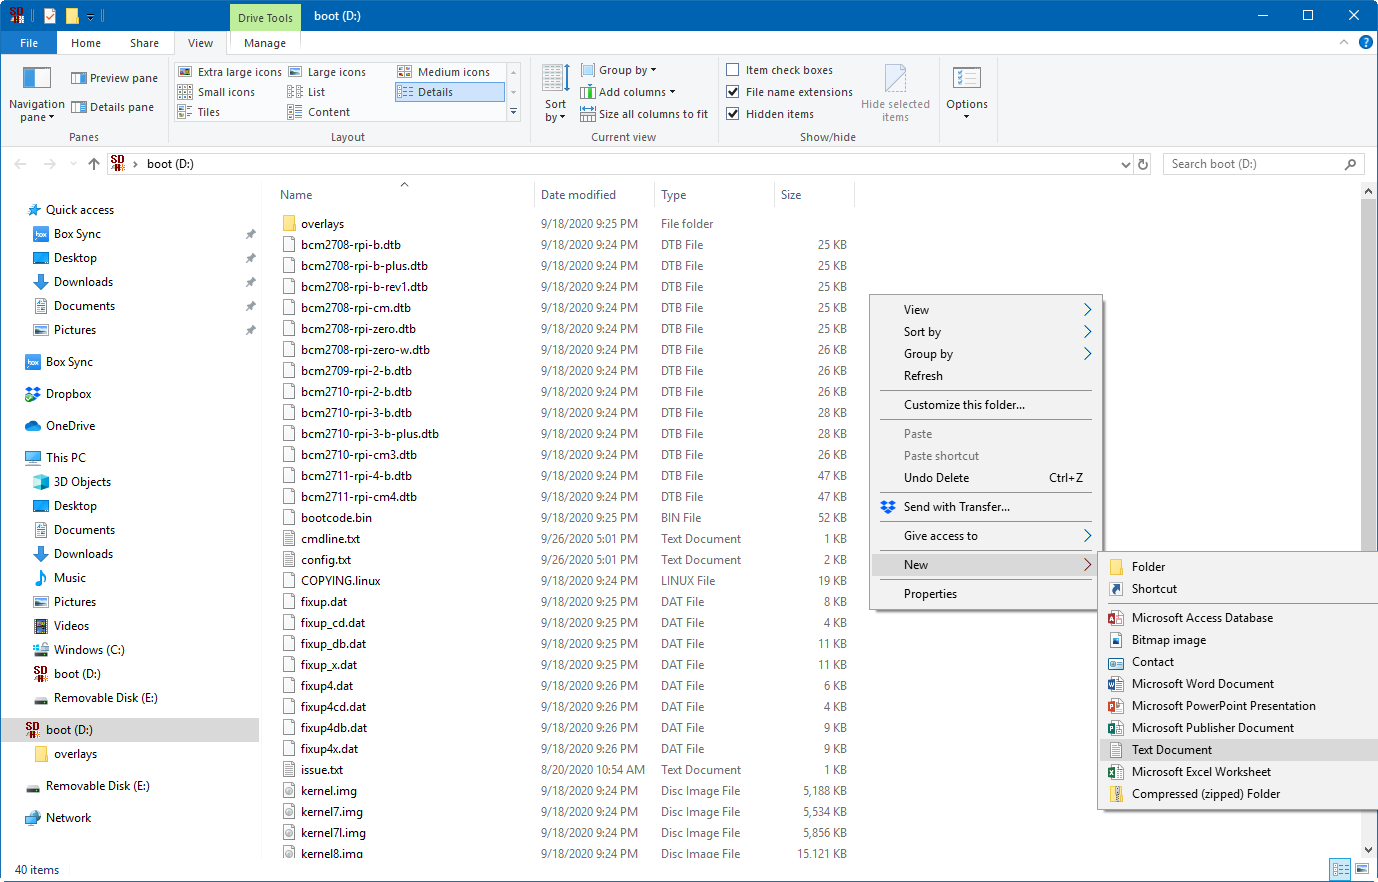
\includegraphics[width=1.00\textwidth]{sdbootnew}
\end{figure}


\begin{figure}
  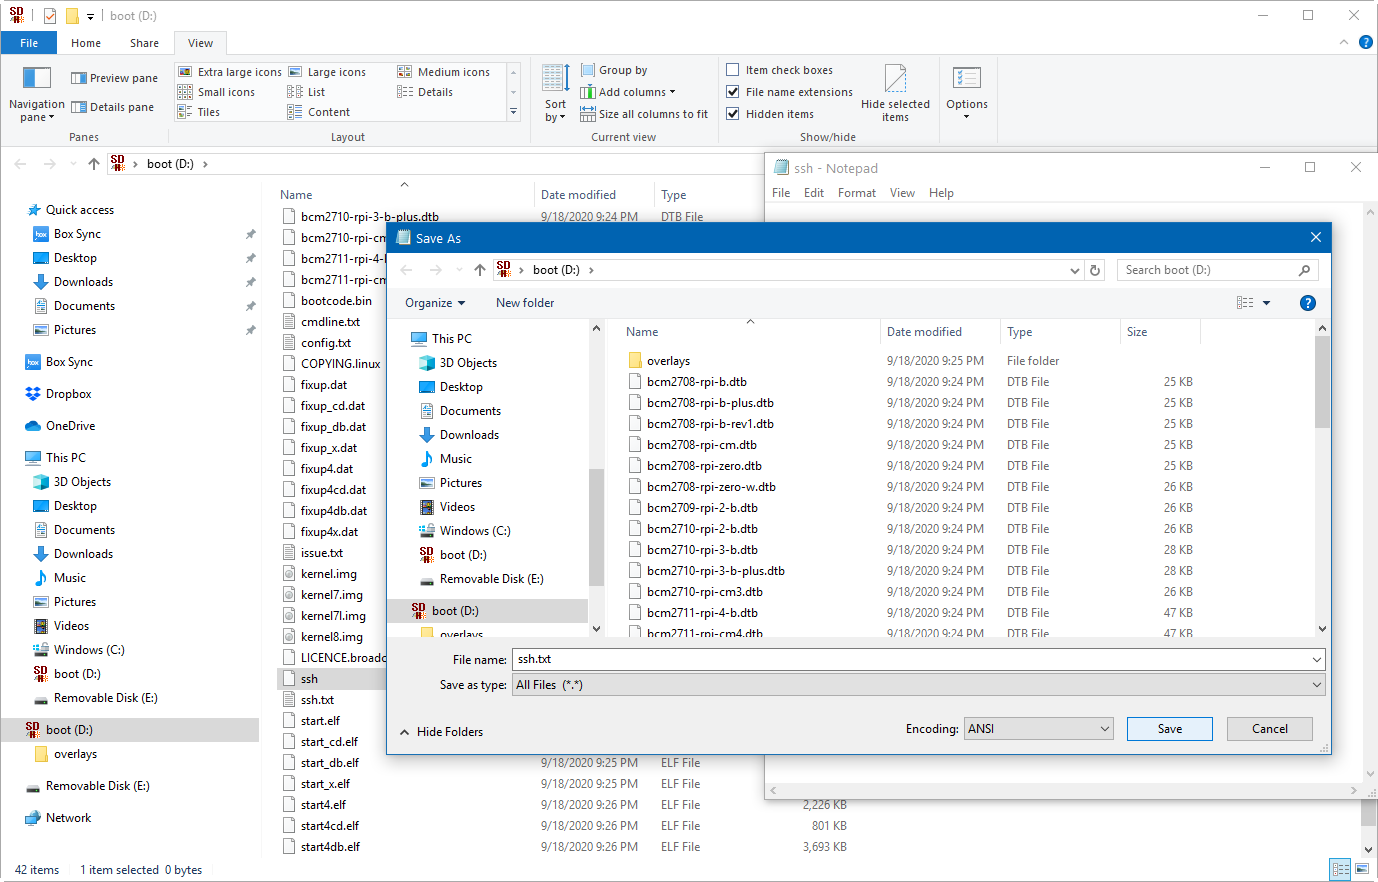
\includegraphics[width=1.00\textwidth]{sdbootaf}
  \caption{.}
  \label{fig:sdbootf}
\end{figure}

  \item You may be promted and asked if you are sure you want to save the file without an extension, select ``Yes.''

\begin{figure}
  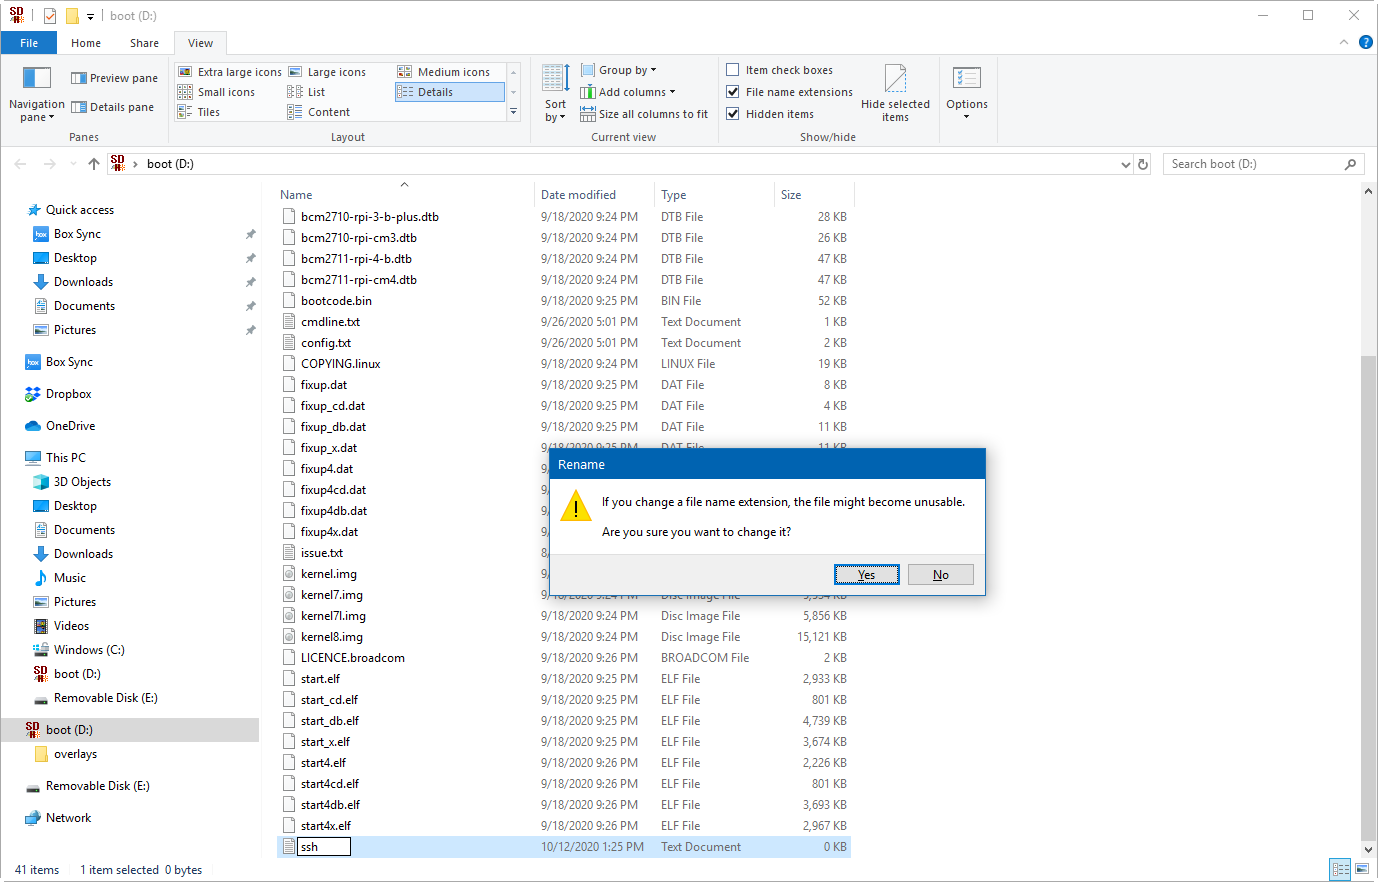
\includegraphics[width=1.00\textwidth]{sdbootays}
  \caption{Saving shh file on a PC.}
  \label{fig:sdbootays}
\end{figure}
  \end{itemize}
  
\clearpage
  
\noindent \textbf{Create wpa\_spplicant.conf file (everone!):}

  \item Using simpler methods as the ''ssh'' file, create and add a file called \textbf{``wpa\_supplicant.conf''} to the boot partition\footnote{where is this?} on the SD card. This can be created with any text editor. %Or you can download a ``template'' from the github \href{https://github.com/marclos/EJnPi/blob/8647e09b3eef07a759606b80e28495be10049813/code/wpa_supplicant.conf}{EJnPi Repository}.
  \begin{itemize}
  \item Make sure the file you created has the \textbf{``.conf''} file extension in the name.
  \item The \textbf{``wpa\_supplicant.conf''} needs to have the WiFi network information in it for the Raspberry Pi to connect on boot up.
  \item Modify this file with a text editor and type the lines below. NOTE: DO NOT COPY AND PASTE. When we copy and paste from other programs hidden text can be inserted that cannot be read by the Pi's operating system correctly.
  \end{itemize}

\begin{lstlisting}
ctrl_interface=DIR=/var/run/wpa_supplicant GROUP=netdev
update_config=1
country=US

network={
 ssid="WIFI NETWORK NAME"
 psk="WIFI PASSWORD"
}
\end{lstlisting}

  \begin{itemize}
  \item If you are not in the United States, input your country's ISO code instead of \textbf{``US''} on the \textbf{\textit{``country=US''}} line.
  \item Make sure to change \textbf{``WIFI NETWORK NAME''} to your WiFi network name, remember this name and password are case senstive.
  \item Make sure to change \textbf{``WIFI\_PASSWORD''} to your WiFi network's password.
  \end{itemize}
  
\end{enumerate}

\subsection{Assemble and Connecting the Pi}

\subsubsection{Putting the Pi together}

\begin{enumerate}
  \item Safely eject the SD card from your main computer.
  \item Place the SD card in the Raspberry Pi Zero W's SD card slot.
  \item Attach the Pi to the bottom Vilros case making sure to line the dowels within the case with the mouting holes on the Pi.
  \item \textbf{Do not} attached the top part of the case yet. Being able to see the Pi's board will help you with pin determination.
  
NOTE: If do not have peripheral devices to be connected to the Pi, i.e. monitor, mouse and keyboard, you will be making a ``headless'' connection and should skip the next few steps. 
\begin{itemize}
  \item Attach your peripheral devices, \textit{if you have them}. This includes a monitor, mouse, and keyboard. It is okay to not have them.
    \item You will need to use the HDMI to micro-HDMI adapter to hook a monitor up to the Raspberry Pi Zero W.
    \item Also, you'll need to use the Anker multiport USB adapter to use a keyboard \textbf{and} a mouse. The Raspberry Pi Zero W only has one micro-usb port.
    \begin{itemize}
     \item You can get away with using just a monitor and keyboard, but if you are not comfortable navigating with a keyboad only, it'll be difficult.
    \end{itemize}
  \end{itemize}
  
  
\item Lastly, making sure the the power adapter for the Pi is plugged in to a power source, and verifying the switch on the adapter is in the \textbf{``off''} position, connect the power cable into the Pi.
  \item Now, turn the power switch on.

\textbf{NOTE!} Make sure not to turn the device off, or on/off/on, otherwise the \textbf{``ssh''} and \textbf{``wpa\_supplicant.conf''} files will not be in your boot directory on the SD card anymore. If, for whatever reason, the Pi loses power after putting those file in the boot directory, you will have to go back and add them, as in step \textbf{\ref{networkssh}}. This is \textbf{especially} important for \textbf{\textit{headless}} users (users with no monitor).

%\textbf{NOTE!} This is where \textbf{\textit{headless}} users will have to remotely connect to the Pi, while people who have monitors, mice, and keyboards won't have to remotely connect. For those who aren't connecting remotely, skip ahead to step \textbf{\ref{updateupgrade}}

\end{enumerate}

\section{Accessing and updating Raspberry Pi OS}

Now, there are different ways to remotely connect with the Raspberry Pi if you are a \textbf{\textit{headless}} user. Unfortunately though, you will have to connect to the Pi using \textbf{SSH} the \textbf{first time}. After that, you can install a remote server on the Pi so you can connect with it using a program with a GUI. I recommend using SSH, though, as it is a \textbf{\textit{much}} quicker connection.

\subsection{Remote connection via SSH}

\subsubsection{Installing Raspberry Pi Finder and finding Pi's IP address}

The goal with this step is to find the \textbf{local IP address} of the Pi. There are a lot of different ways to do this. If you are computer savvy, go ahead and find the IP address of your Pi and ingnore this step.

\begin{enumerate}
  \item The easiest way to find the IP address of your Pi, if you don't know networking or computers that well, is to use the \textbf{Raspberry Pi Finder} by Adafruit. 
  \item With your main computer, go to this website to download the application for your OS: \newline \newline \url{https://github.com/adafruit/Adafruit-Pi-Finder/}.\newline \newline
\textbf{Note for Mac users}: If you are prevented from launching the app because of your security settings, you can right click on the app and click Open to bypass the warnings.
  \item However, if this doesn't work, try this: \newline \newline \url{http://ivanx.com/ivanx/raspberrypi/}. \newline \newline If this program works, follow the instructions and skip to Section \ref{updateupgrade}. 
  
  \item Scroll down and click the link that says \textbf{``Download the latest release''}
  \item Scroll down to \textbf{``Assets''} and there you will see the .zip files of the program for the different OSs.
  \begin{itemize}
    \item \textbf{``osx''} is for Mac users.
    \item \textbf{``win32''} is for Windows user.
  \end{itemize}
  \item Download the .zip file for your system and then unzip it when finished downloading.
  \item Run Raspberry Pi finder by double-clicking \textbf{``PiFinder.exe''}, which is in the folder you just unzipped.
  \item Click \textbf{``Find my Pi!''} for the program to locate your Pi. Wait a few minutes if it doesn't find it immediately. Sometimes it can take quite a while!\footnote{need a workaround, this doesn't work...}
  \item The IP address should be listed when finished. It should look something like \textbf{``192.168.1.XXX''}. \label{ipaddress}
  \item Use the IP address to connect to the Pi.
\end{enumerate}

\subsubsection{SSH connection}
\label{ssh}

\begin{itemize}
    \item For Windows users, you will want to use the \textbf{Command Prompt}.
    \begin{enumerate}
      \item Press the \textbf{\textit{Windows}} key on your keyboard, type \textbf{``CMD''}, and \textbf{Enter}.
\newline
\newline
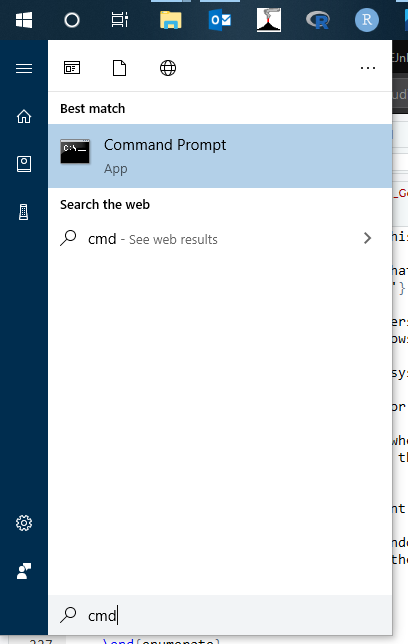
\includegraphics[scale=0.70]{cmd}
      \item In the Command Prompt, type the command below making sure to substitute ``192.168.0.XXX'' with the IP address found in step \ref{ipaddress}
      \begin{lstlisting}
      ssh pi@192.168.0.XXX 
      \end{lstlisting}
      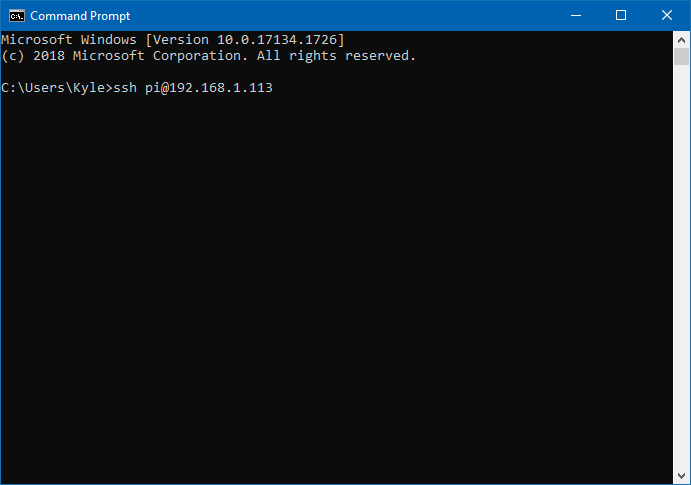
\includegraphics[width=1.00\textwidth]{cmdssh}
    \end{enumerate}
    \item For Mac users, you will want to use the \textbf{\textit{Terminal}}.
    \begin{enumerate}
      \item Press the \textbf{\textit{Command + Spacebar}} keys on your keyboard, type \textbf{``Terminal''}, and \textbf{Enter}.
  \newline
  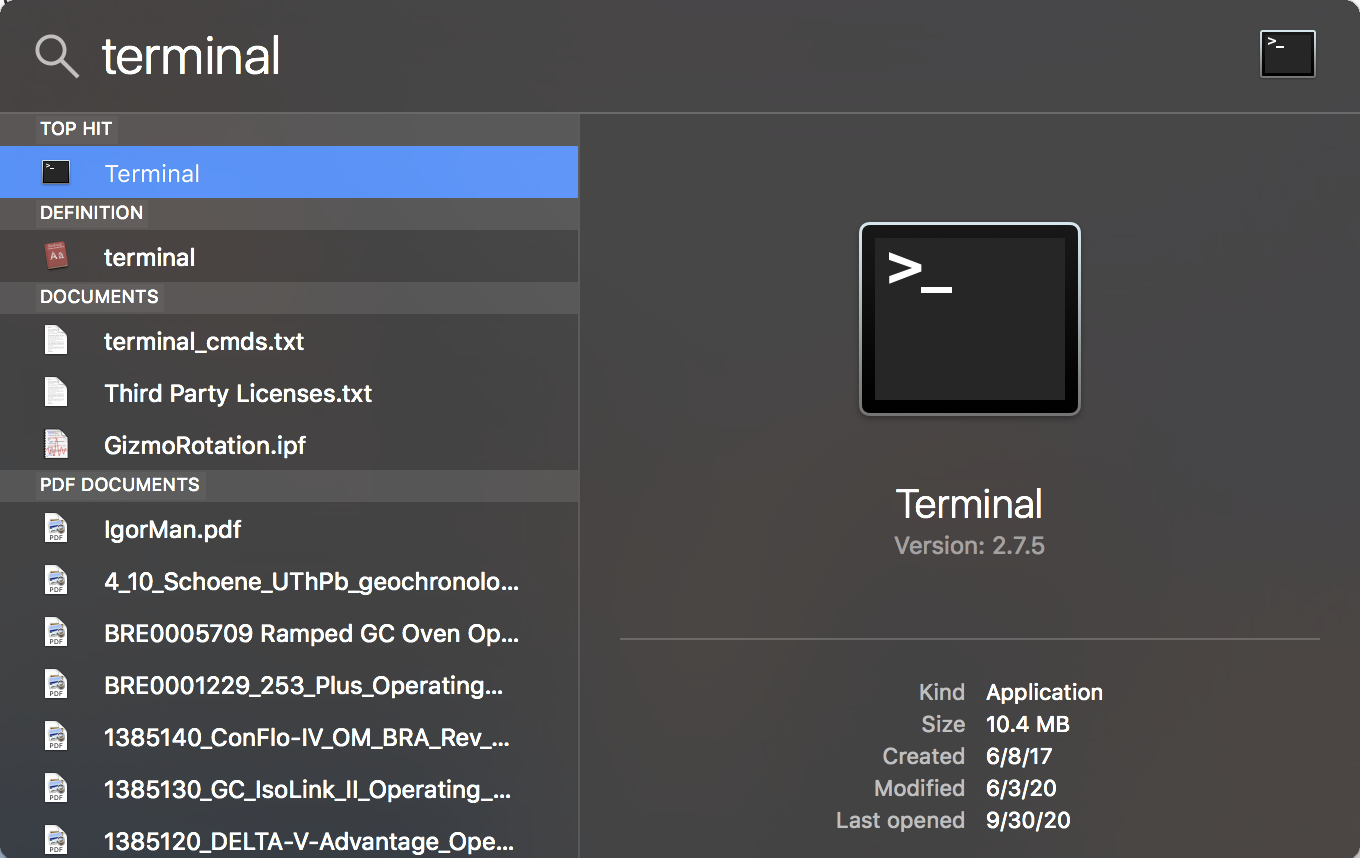
\includegraphics[width=1.00\textwidth]{searchterm}
  \newline
      \item In Terminal, type the command below making sure to substitute ``192.168.1.XXX'' with the IP address found in step \ref{ipaddress}.
      \begin{lstlisting}
      ssh pi@192.168.1.XXX 
      \end{lstlisting}
  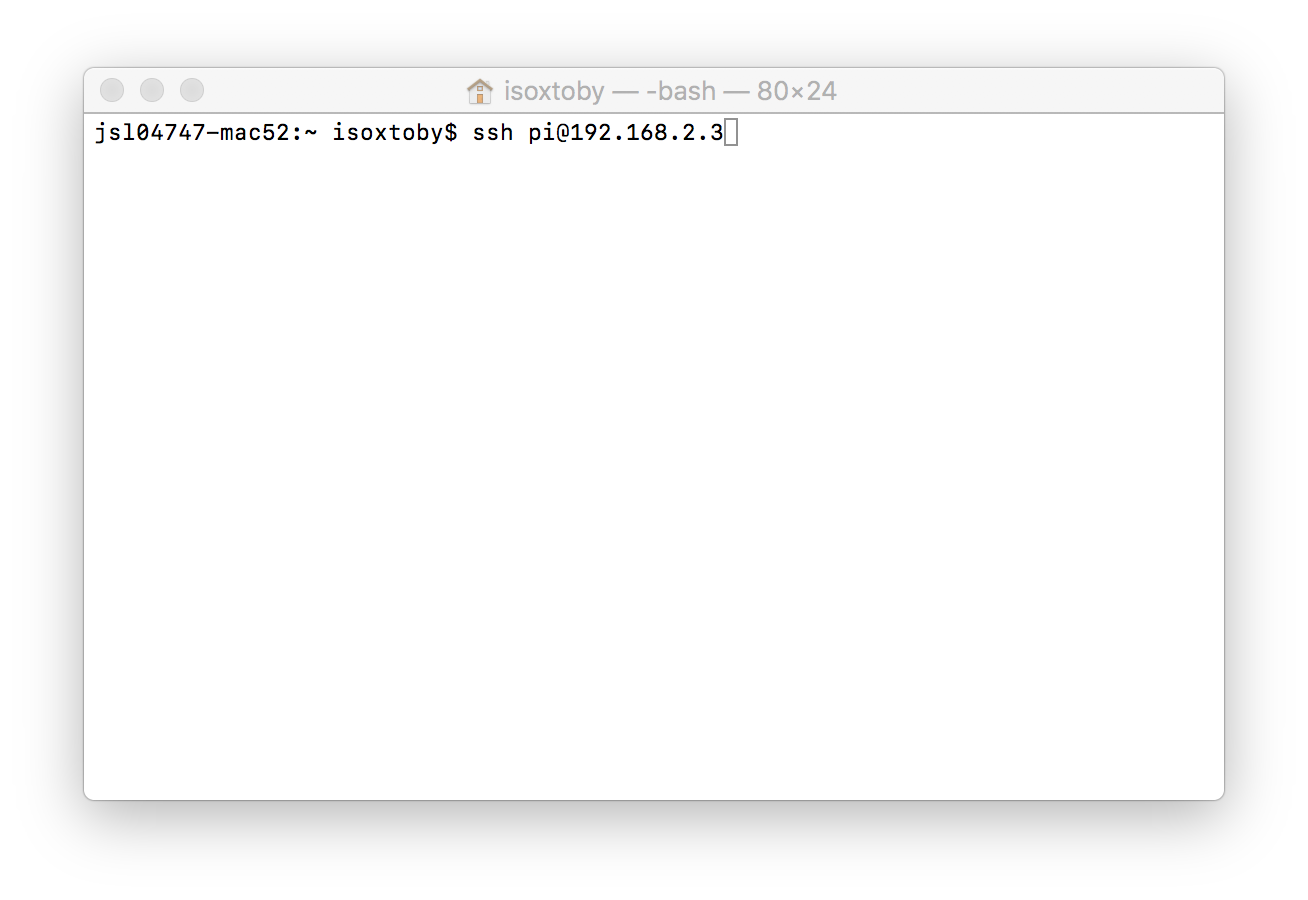
\includegraphics[width=1.00\textwidth]{termssh}
    \end{enumerate}
    
NOTE: Sometimes we get a warning that the host key needs to be changed. If you get a yes/no prompt, type yes. If you get a warning that the key needs to be changed or that someone is snooping then contact the instructor for help with this.  
\end{itemize}
\begin{enumerate}
  \item For both Mac and Windows users, you should now see a prompt in the command line asking for the Pi's password.
  \newline
  \newline
  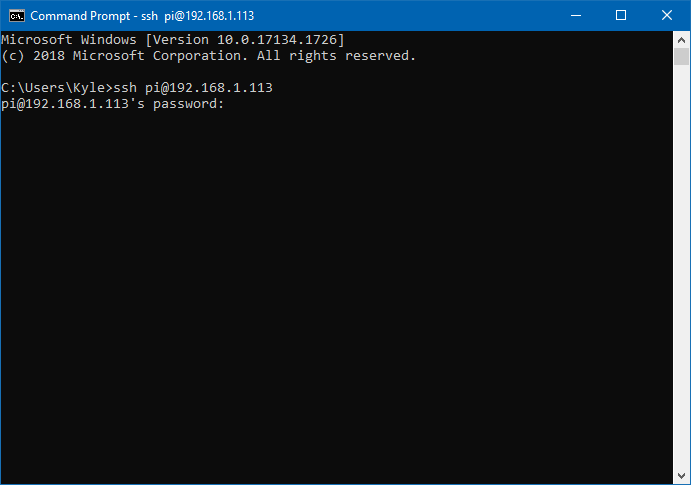
\includegraphics[width=1.00\textwidth]{cmdsshpw}
  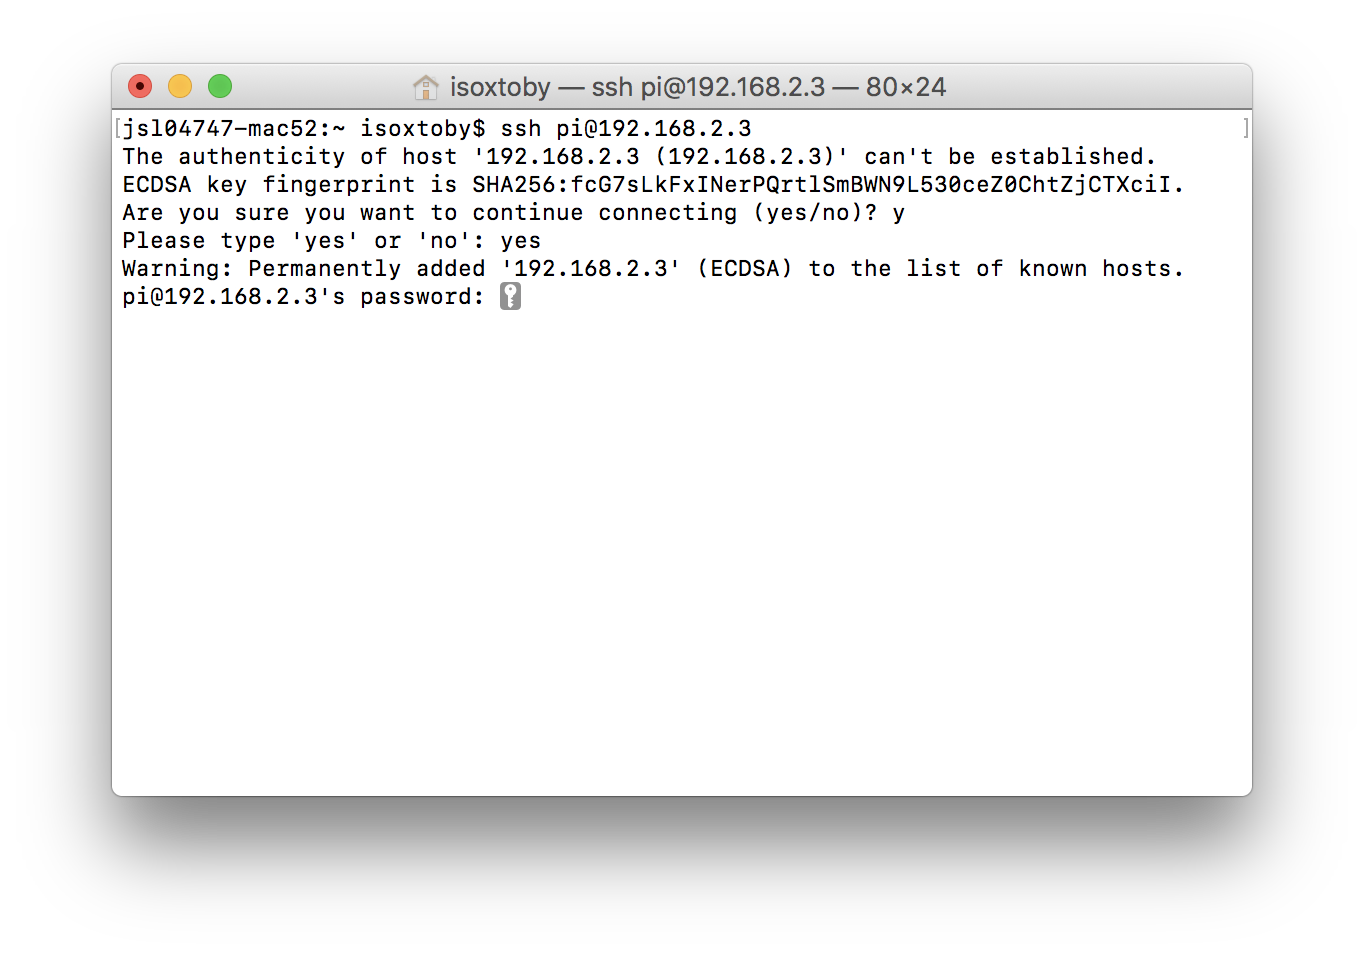
\includegraphics[width=1.00\textwidth]{termsshpw}
  \newline
  \newline
  By default, the password is \textbf{``raspberry''}. 
  \newline 
  \newline 
  \textbf{NOTE} The command line won't show the password while you are typing it, nor will it show placeholder characters. You will need to just type it and \textbf{Enter}.
  \item If all went well, you should see that you've connected to your Pi via the command line interface (CLI). You should see the text: 
  \begin{lstlisting}
  pi@raspberrypi/:~ $_ 
  \end{lstlisting}
  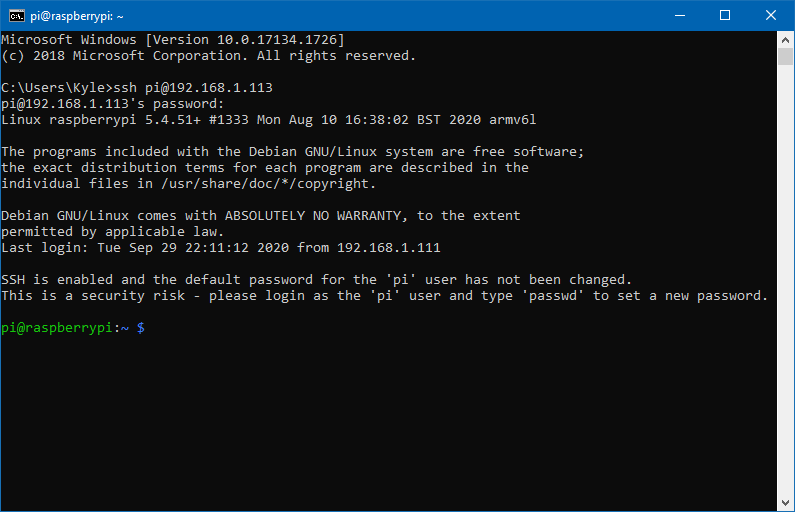
\includegraphics[width=1.00\textwidth]{cmdsshrp}
  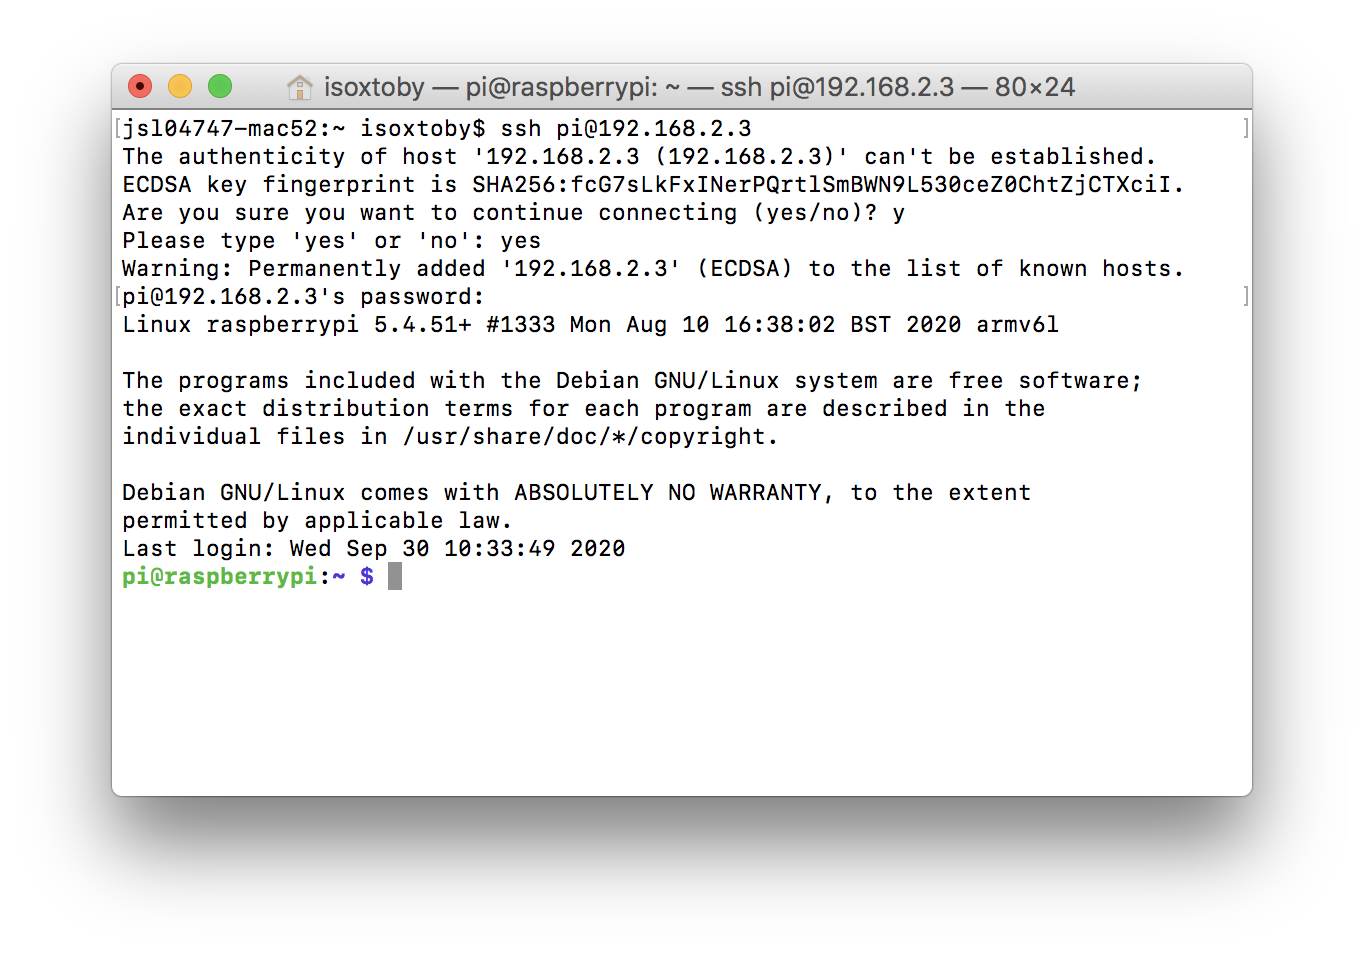
\includegraphics[width=1.00\textwidth]{termsshpwconf}
  \item There will also be a warning that the Pi's password hasn't been changed. We will want to change that, but we are not going to do that right now.
\end{enumerate}

\subsection{Update and Upgrading Raspberry Pi OS} 
\label{updateupgrade}

Here we will be updating the Raspberry Pi. This is the first thing we are going to want to do to make sure there are now errors later on. We will need to implement a few commands into the Pi's command line. Don't be afraid! Its easy!

\begin{enumerate}
  \item First we are going to want the Pi to talk to the official Raspberry Pi servers to get the latest version list of our programs on the Pi. In your SSH session, type the following command:
  \begin{lstlisting} 
  sudo apt update
  \end{lstlisting}
  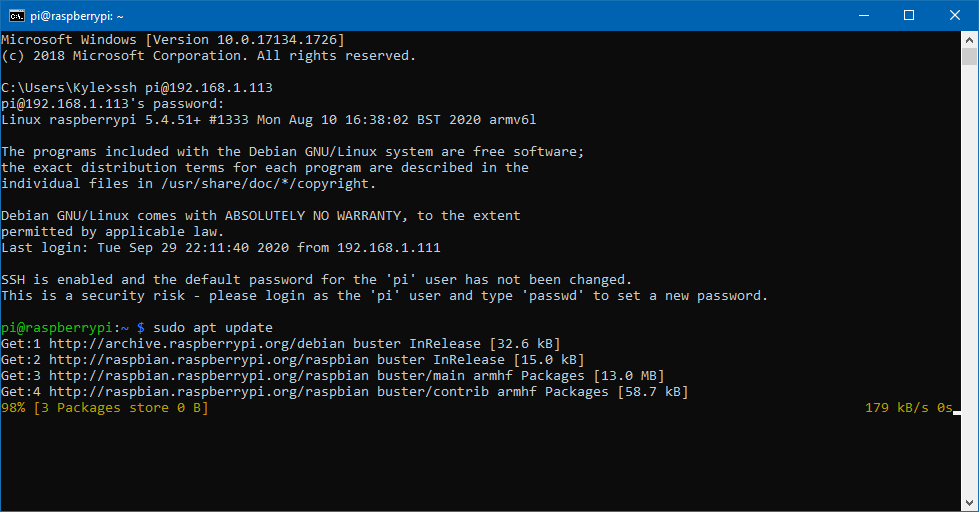
\includegraphics[width=1.00\textwidth]{aptupdate}
  \item Secondly, we want the Pi to compare the version list with its current packages and programs and update where needed. In your SSH session, type:
  \begin{lstlisting}
  sudo apt full-upgrade
  \end{lstlisting}
  \item You will be asked if you are sure you want to upgrade. Type \textbf{``y''} and \textbf{Enter}.
  \newline
  \newline
  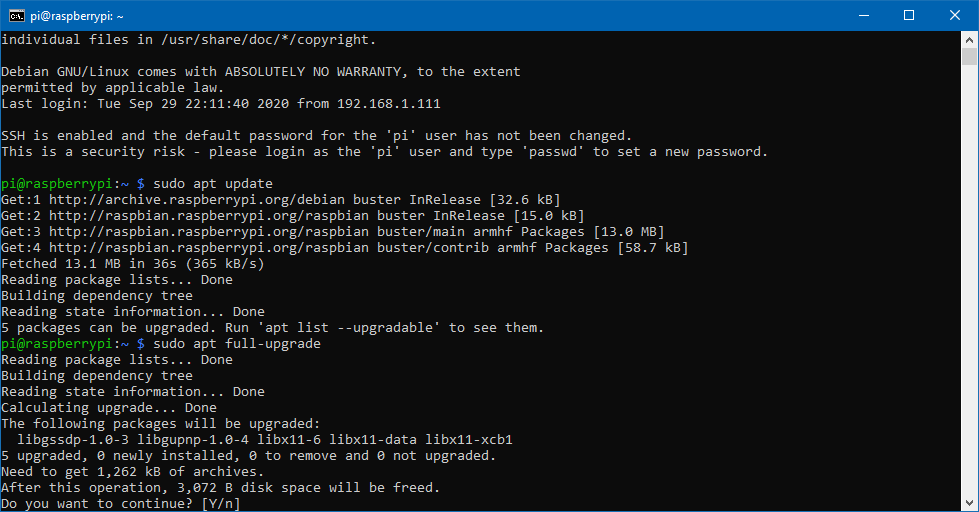
\includegraphics[width=1.00\textwidth]{aptupgradecont}
  \item Once it is finished, it will show this once again:
  \begin{lstlisting}
  pi@raspberrypi/:~ $_ 
  \end{lstlisting}
  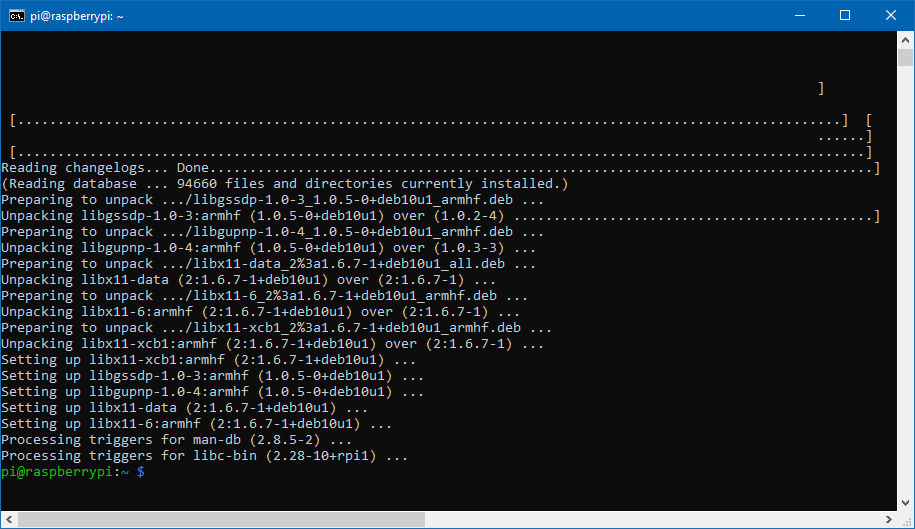
\includegraphics[width=1.00\textwidth]{aptupgradedone}
  \item Congratulations! Your Pi has been upgraded!
\end{enumerate}

\section{Configuring the Pi}

\begin{itemize}
  \item Hopefully you still have your current SSH connection going with your Pi. If not, try to create one. If you exited the Command Prompt/Terminal, and severed the SSH connection, just reopen them and reconnect via SSH as in step \ref{ssh}.
  \item If \textbf{power} was severed from the Pi, you will need to repeat section \ref{networkssh} over again. The Pi discards these files after it boots up, so if you shut off the Pi, or lose power, you'll have to re-add them to the boot directory.
\end{itemize}

\subsection{Changing the Pi User Password}

As a security measure, since your Pi is in your WiFi network, you'll want to change the password for the Pi.

\begin{enumerate}
  \item Run the Raspberry Pi configuration utility by using this command in the CLI:
  \begin{lstlisting}
  sudo raspi-config
  \end{lstlisting}
  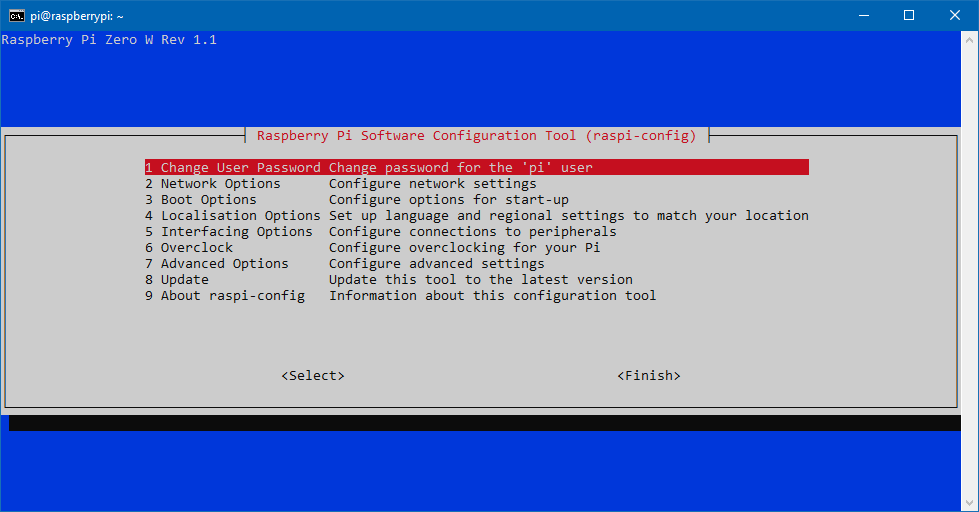
\includegraphics[width=1.00\textwidth]{rcpw}
  \item Navigate to \textbf{``Change User password for the 'pi' user''} and hit \textbf{Enter}.
  \item It will prompt you that it is going to ask for the new password. Press \textbf{Enter}, and type your new password followed by \textbf{Enter} again.
  \newline
  \newline
  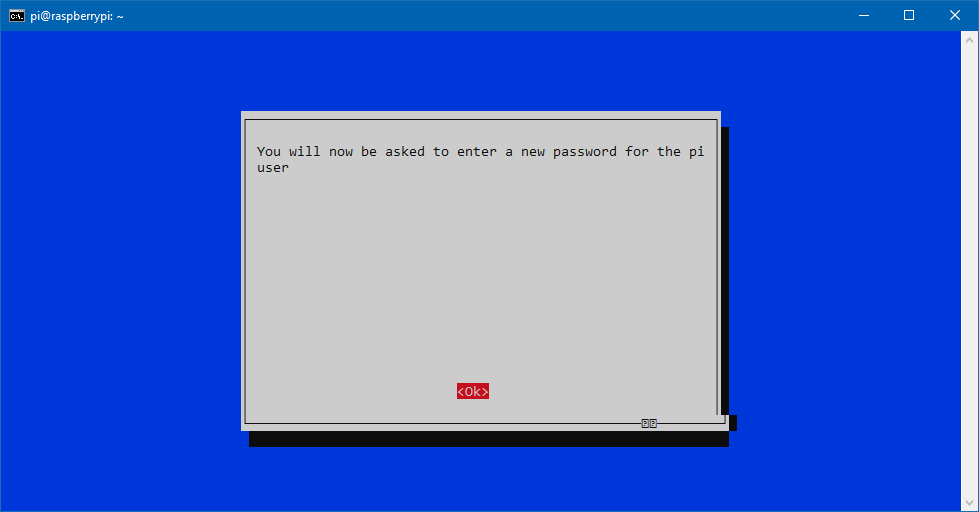
\includegraphics[width=1.00\textwidth]{rcpwconf}
  \item Verify the password by typing it again.
  \newline
  \newline
  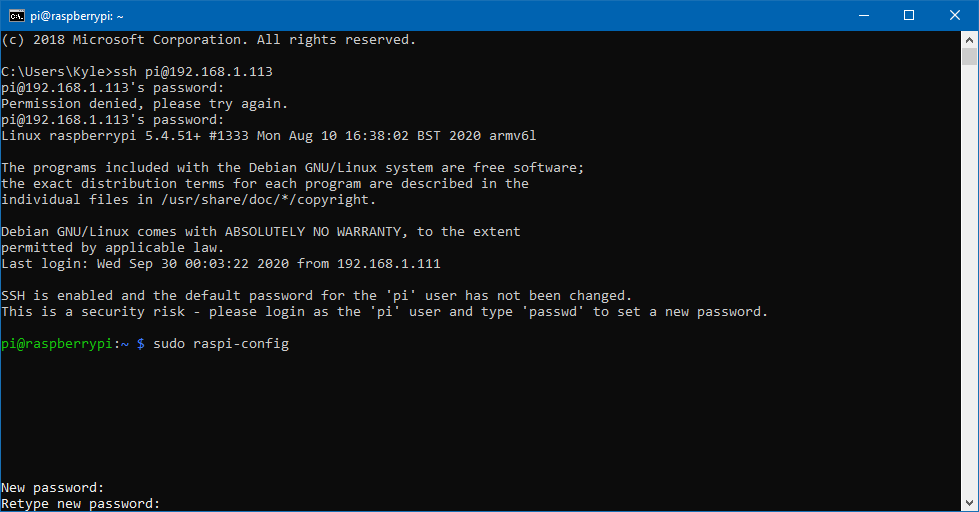
\includegraphics[width=1.00\textwidth]{rcpwretype}
  \item Your Pi now has your new password. Don't forget it!
\end{enumerate}

\subsection{Network Options}

We want to make sure the Pi's network options are configured properly so we don't have to add a \textbf{wpa\_supplicant.conf} file to the boot directory when booting anymore.

\begin{enumerate}
  \item While still in the raspi-config utility, navigate to \textbf{``Network Options''}.
  \newline
  \newline
  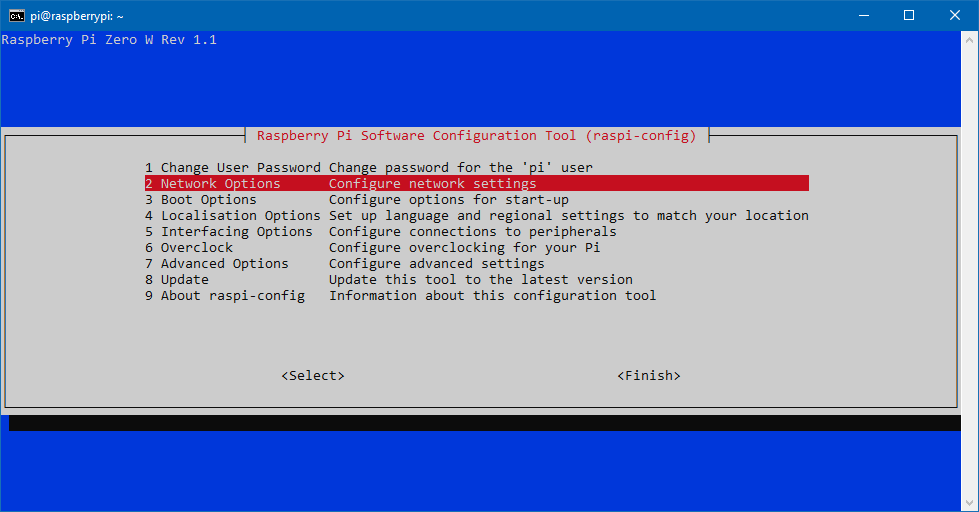
\includegraphics[width=1.00\textwidth]{rcnet}
  \item Navigate to \textbf{``Wireless LAN''} and hit \textbf{Enter}.
  \newline
  \newline
  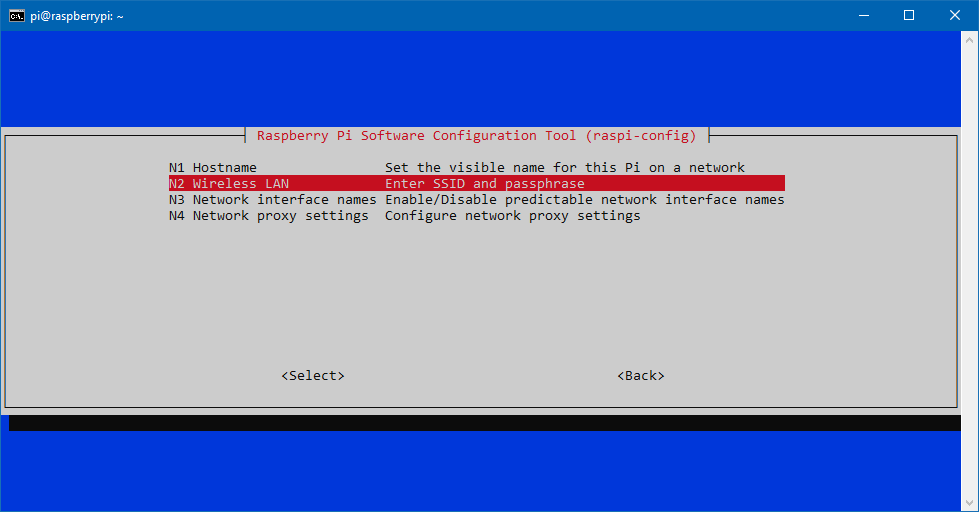
\includegraphics[width=1.00\textwidth]{rcnetwlan}
  \item It will prompt you to enter your WiFi \textbf{SSID}. This is the name of the WiFi network. Enter it and press \textbf{Enter}.
  \newline
  \newline
  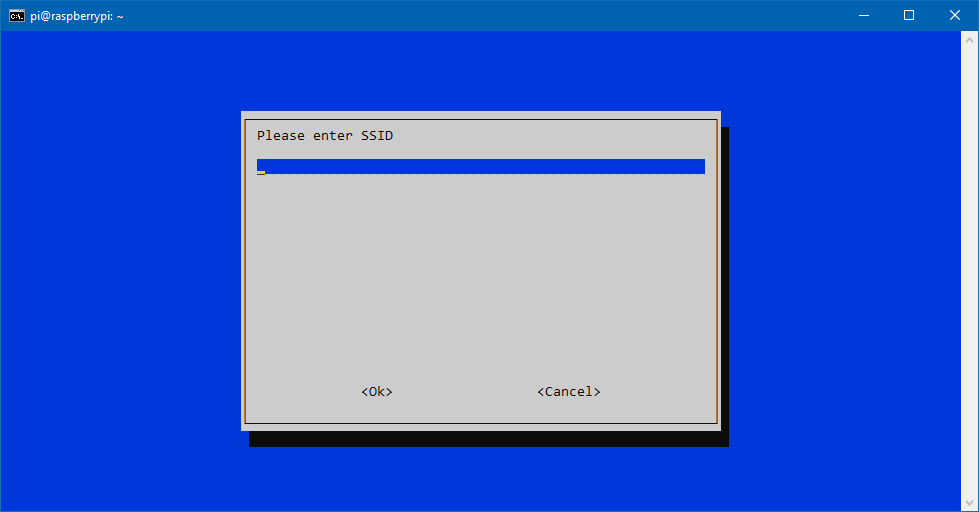
\includegraphics[width=1.00\textwidth]{rcnetwlanssid}
  \item Next it will ask for the WiFi password/passphrase. Type that in and hit \textbf{Enter}.
  \newline
  \newline
  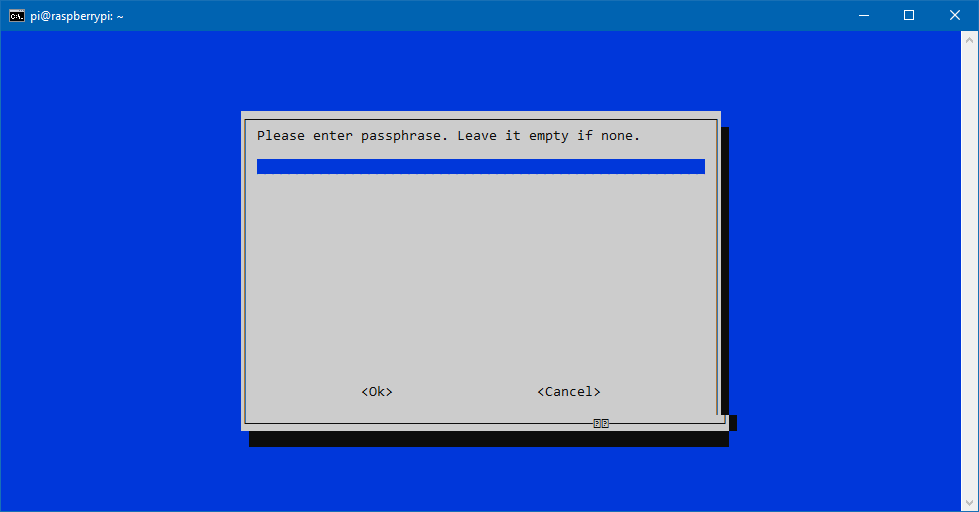
\includegraphics[width=1.00\textwidth]{rcnetwlanpw}
  \item If done correctly, it will notify you it was successfully done via the CLI.
  \newline
  \newline
  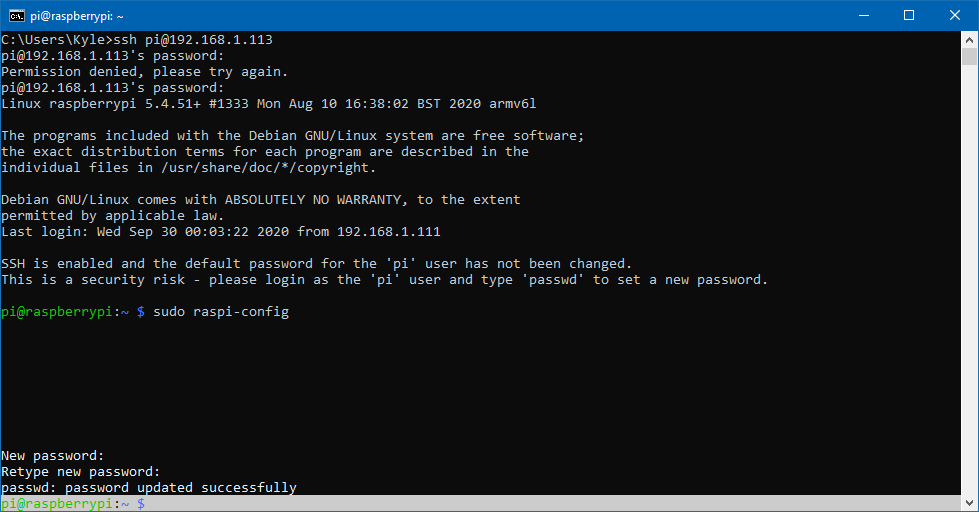
\includegraphics[width=1.00\textwidth]{rcnetwlansuccess}
  \item Your Pi now has the wireless network configured properly.
\end{enumerate}

\subsection{Boot Options}

This next configuration is more for fun and is \textbf{OPTIONAL}. We are going to make the Raspberry Pi \textbf{``text boot''} instead of just showing a splash screen. This is fun because it shows you the boot process via the CLI so you can see \textbf{\textit{exactly}} what is starting during boot up!

\begin{enumerate}
  \item While still in the raspi-config utility, navigate to \textbf{``Boot Options''}.
  \newline
  \newline
  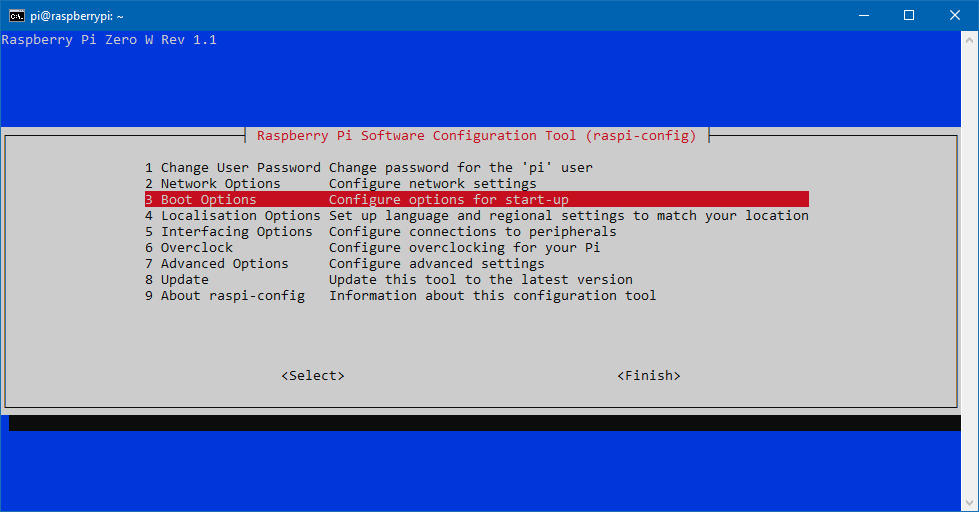
\includegraphics[width=1.00\textwidth]{rcboot}
  \item Navigate to \textbf{``Splash Screen''}.
  \newline
  \newline
  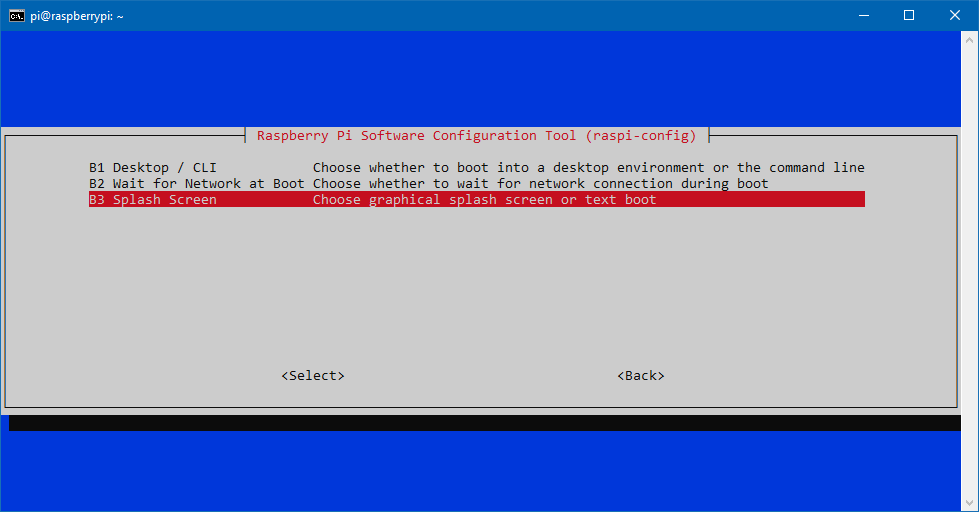
\includegraphics[width=1.00\textwidth]{rcboottext}
  \item It will prompt you if you want to see the \textbf{splash screen} at boot. Select \textbf{``NO''}
  \newline
  \newline
  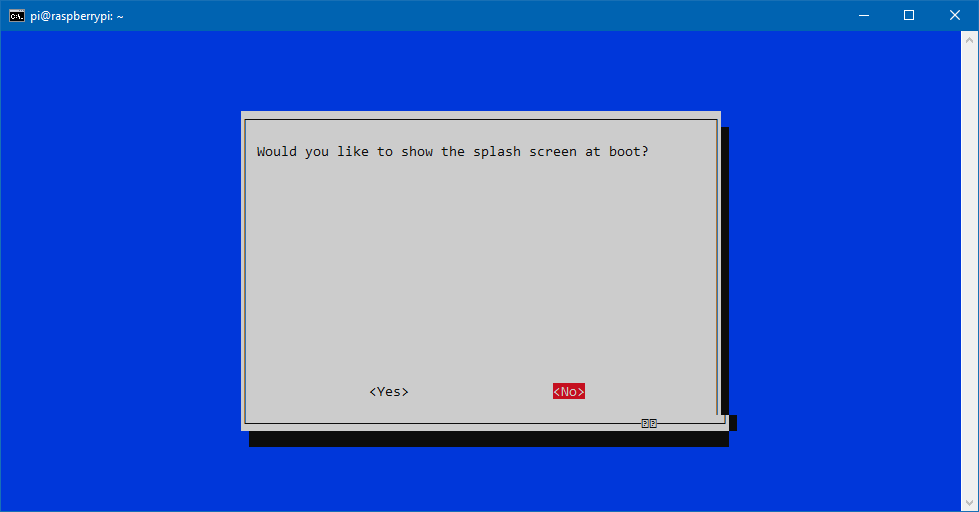
\includegraphics[width=1.00\textwidth]{rcboottextconf}
  \item It will then tell you that the splash screen at boot is disabled. Woohoo!
\end{enumerate}

\subsection{Localization Options}

This may or may not be a problem for some people. I had to make sure my time zone was set correctly. I believe by default the Pi's time zone is set for Europe.

\begin{enumerate}
  \item While still in the raspi-config utility, navigate to \textbf{``Localisation Options''}.
  \newline
  \newline
  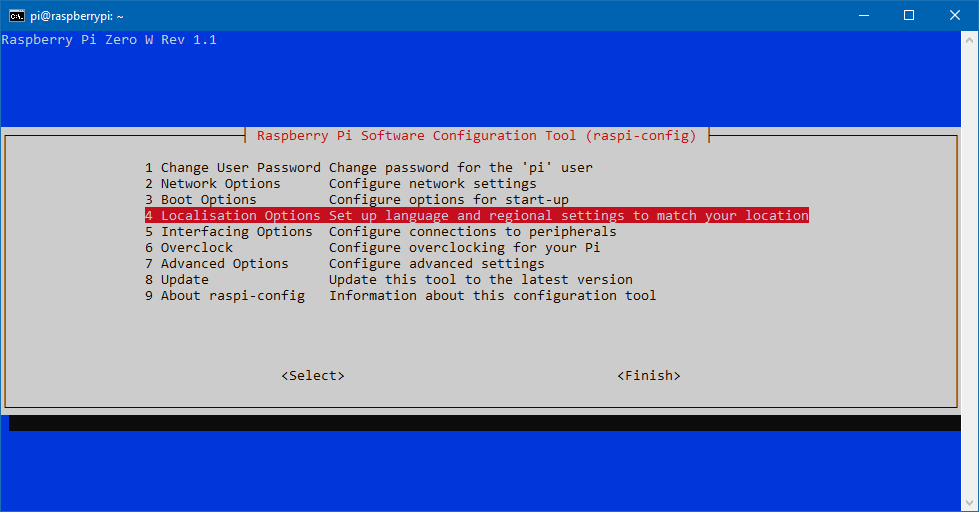
\includegraphics[width=1.00\textwidth]{rclocale}
  \item Navigate to \textbf{``Change Time Zone''}.
  \newline
  \newline
  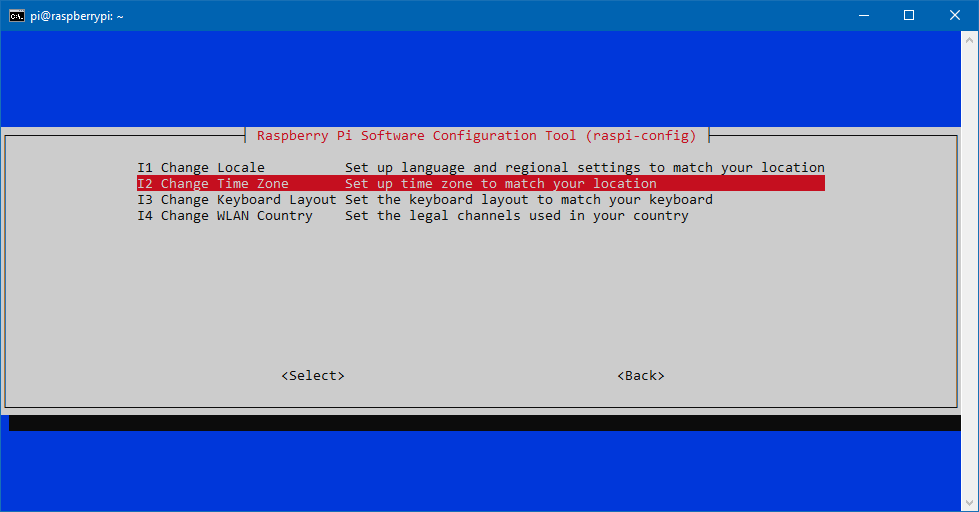
\includegraphics[width=1.00\textwidth]{rctime}
  \item In a few seconds it will prompt you to choose your \textbf{geographic area}. Select whichever corresponds to yours. In my case it was the US.
  \newline
  \newline
  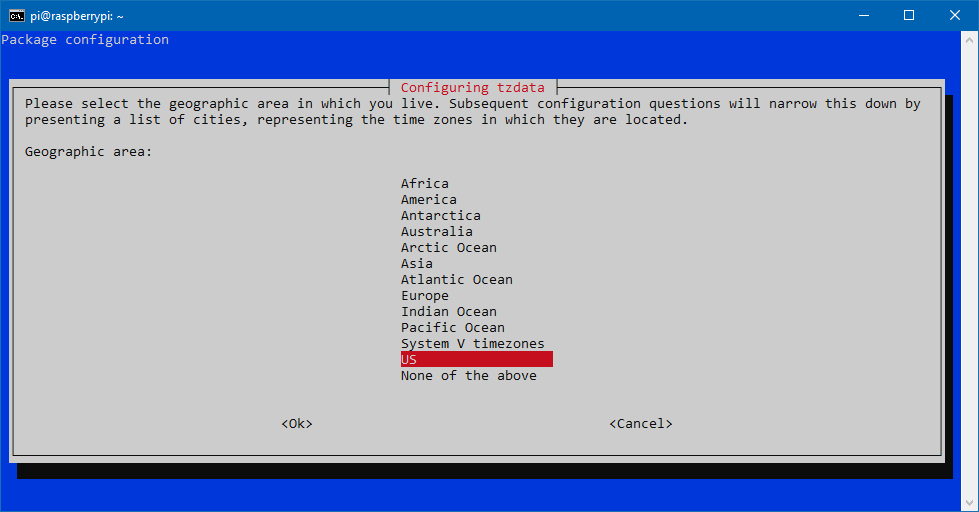
\includegraphics[width=1.00\textwidth]{rctimeus}
  \item It will then tell ask you what  your \textbf{time zone} is. Select what applies. In my case is was Pacific Ocean.
  \newline
  \newline
  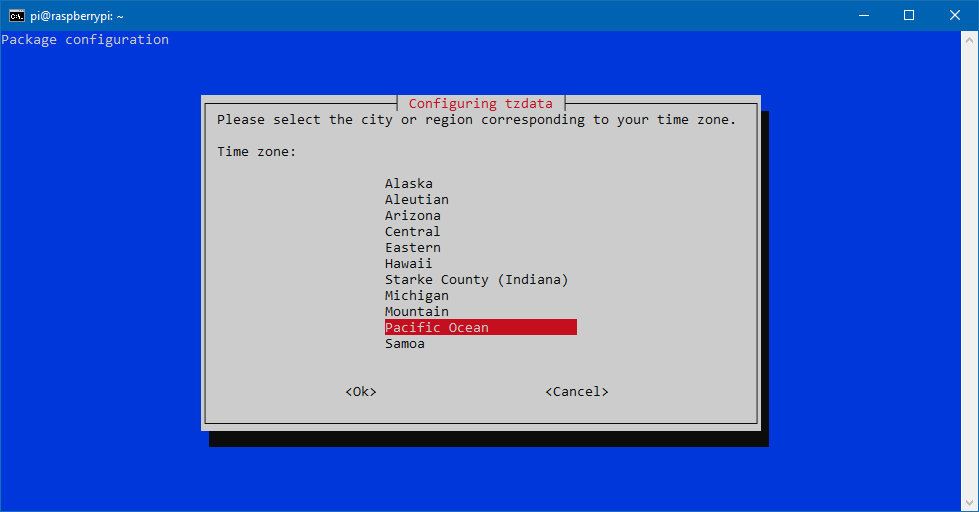
\includegraphics[width=1.00\textwidth]{rctimepo}
  \item Then, it will flash the CLI with the Coordinated Universal Time (UTC) and your time zone's time and go back to the configuration utility.
\end{enumerate}

\subsection{Interfacing Options (enable SSH)}

\textbf{IMPORTANT} We need to make sure we enable SSH in the Pi's configuration. This is extremely important and allows us to connect to the Pi via SSH in all future instances without having to add a ssh file to the boot directory.

\begin{enumerate}
  \item While still in the raspi-config utility, navigate to \textbf{``Interfacing Options''}. Remember where this is located because we will need to access this later on.
  \newline
  \newline
  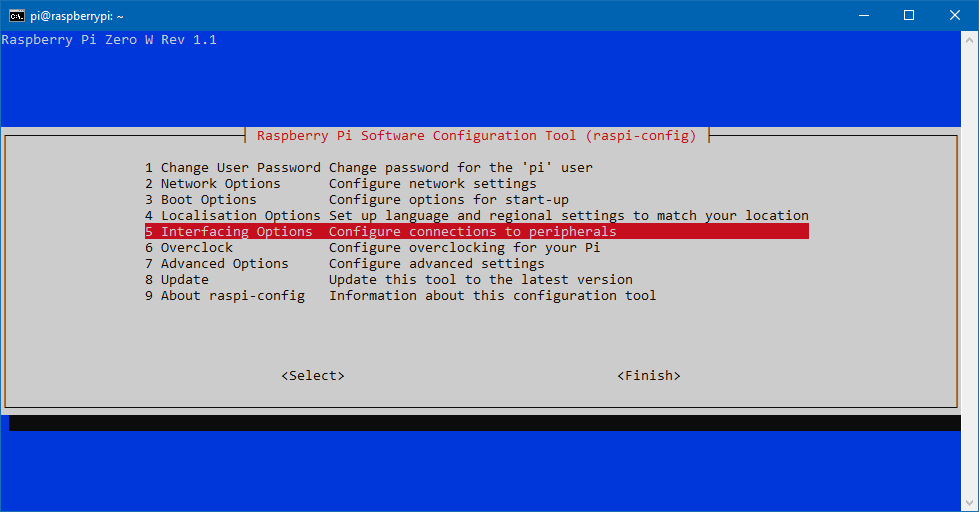
\includegraphics[width=1.00\textwidth]{rcifoptions}
  \item Navigate to \textbf{``SSH''}.
  \newline
  \newline
  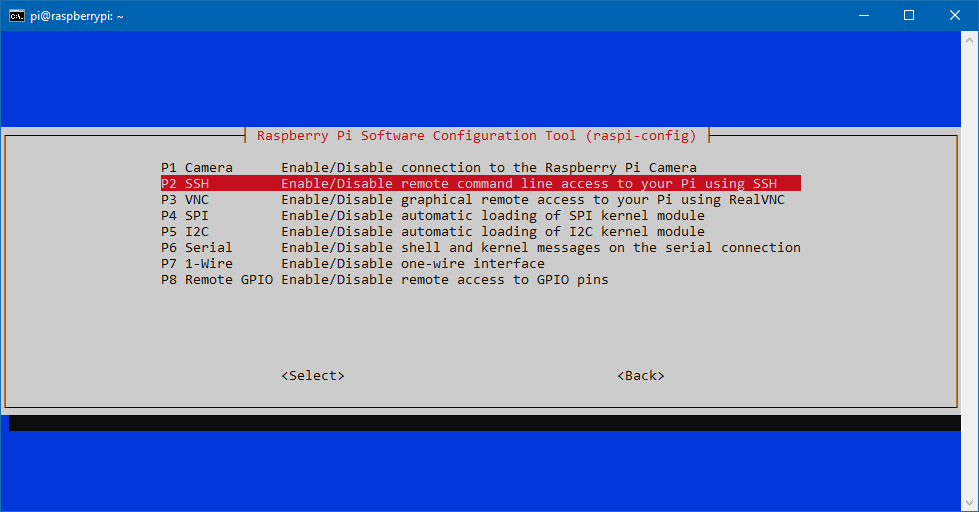
\includegraphics[width=1.00\textwidth]{rcssh}
  \item The Pi will then ask if you want the \textbf{SSH server} enabled. Select \textbf{Yes}.
  \item Wait a few seconds and the Pi should notify you the SSH server is enabled.
\end{enumerate}

\subsection{Virtual Network Computing (VNC) Option}

\textbf{NOTE} For those who find the CLI a bit tricky, or just don't like it, you can enable a virtual network computing software called RealVNC before shutting down the Pi. This will let you control the Pi via a graphical user interface (GUI), like what people are normally used to on MacOS or Windows.

\begin{enumerate}
  \item While still in the raspi-config utility, navigate to \textbf{``Interfacing Options''}.
  \newline
  \newline
  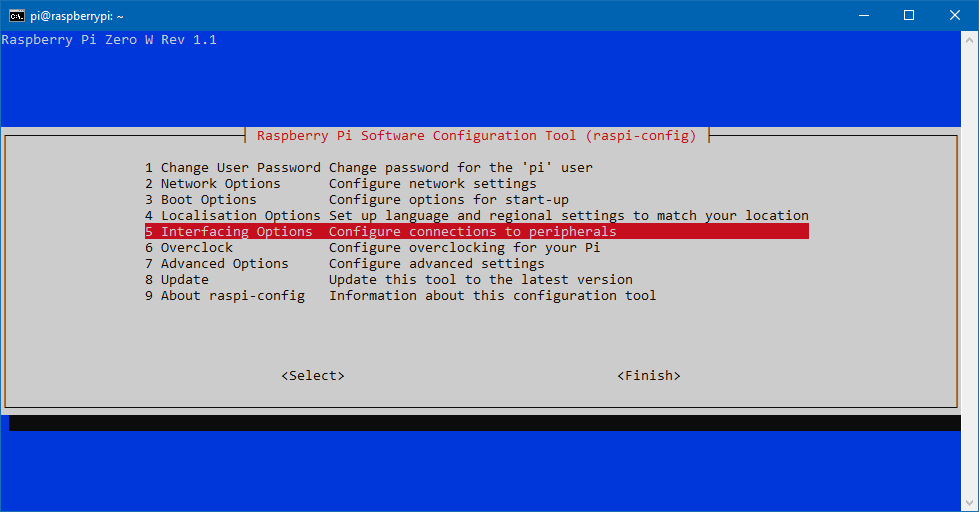
\includegraphics[width=1.00\textwidth]{rcifoptions}
  \item Navigate to \textbf{``VNC''} and select it.
  \newline
  \newline
  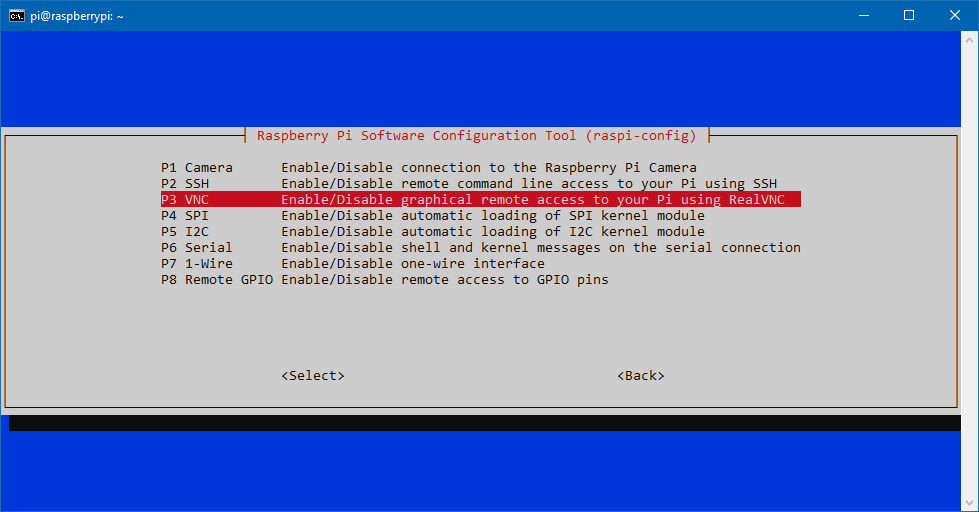
\includegraphics[width=1.00\textwidth]{rcvnc}
  \item The Pi will prompt you if you want the \textbf{VNC Server} enabled. Select \textbf{``Yes''}.
  \newline
  \newline
  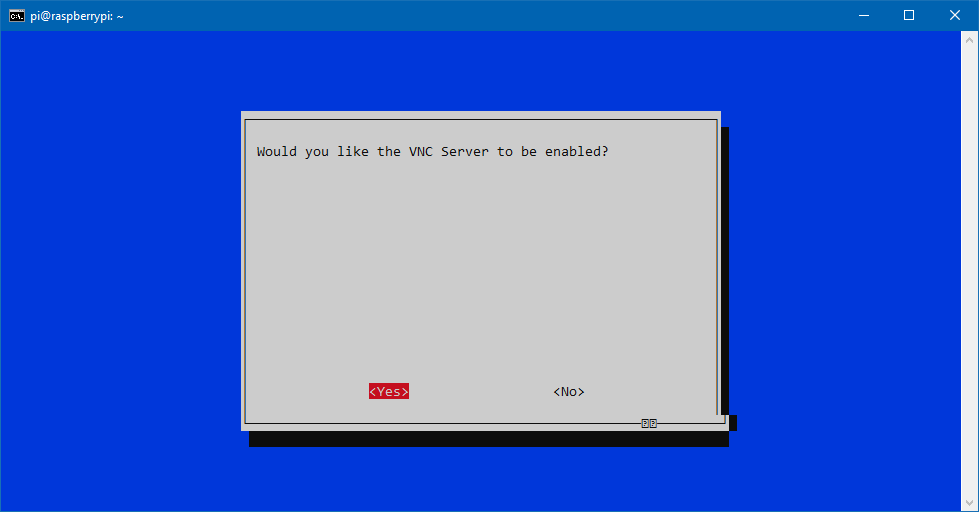
\includegraphics[width=1.00\textwidth]{rcvncenable}
  \item Wait a second and the Pi should let you know that the \textbf{VNC Server} is now enabled. This server will start automatically when the Pi boots up.
  \newline
  \newline
  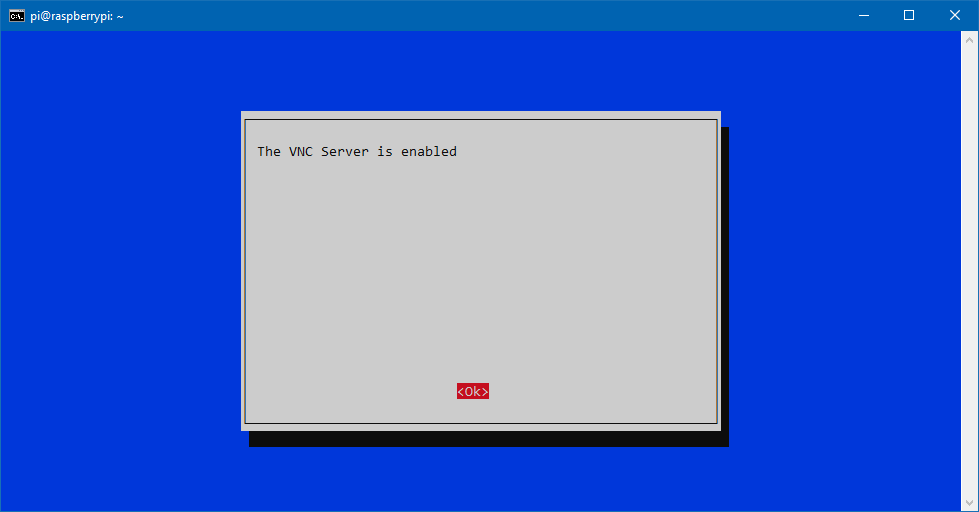
\includegraphics[width=1.00\textwidth]{rcvncconf}
  \item You still need to download \textbf{RealVNC} \textbf{\textit{Viewer}} on the computer you want to remotely access the Pi with.
  \item \textbf{RealVNC Viewer} can be downloaded at:
  \newline
  \url{https://www.realvnc.com/en/connect/download/viewer/}\footnote{I don't think this will work -- I prefer using remote desktop connection... why did you pick this one?} \footnote{Raspberry Pi OS comes with RealVNC Server already installed, you just have to enable the option (covered in the SOP). The other requirement is that you download RealVNC Viewer on the computer you want to VNC in with. I chose this route because it already is sort of equipped with RasPi OS, and the Viewer is cross-platform so I wouldn't need to write two sections of the SOP, on OSX and Windows.}
  \item Download the client that is for your OS and then install it.  
  \item When you open VNC Viewer, you should see something like the image below. In the top toolbar, input the IP address of the Pi and hit \textbf{``Enter''}.
  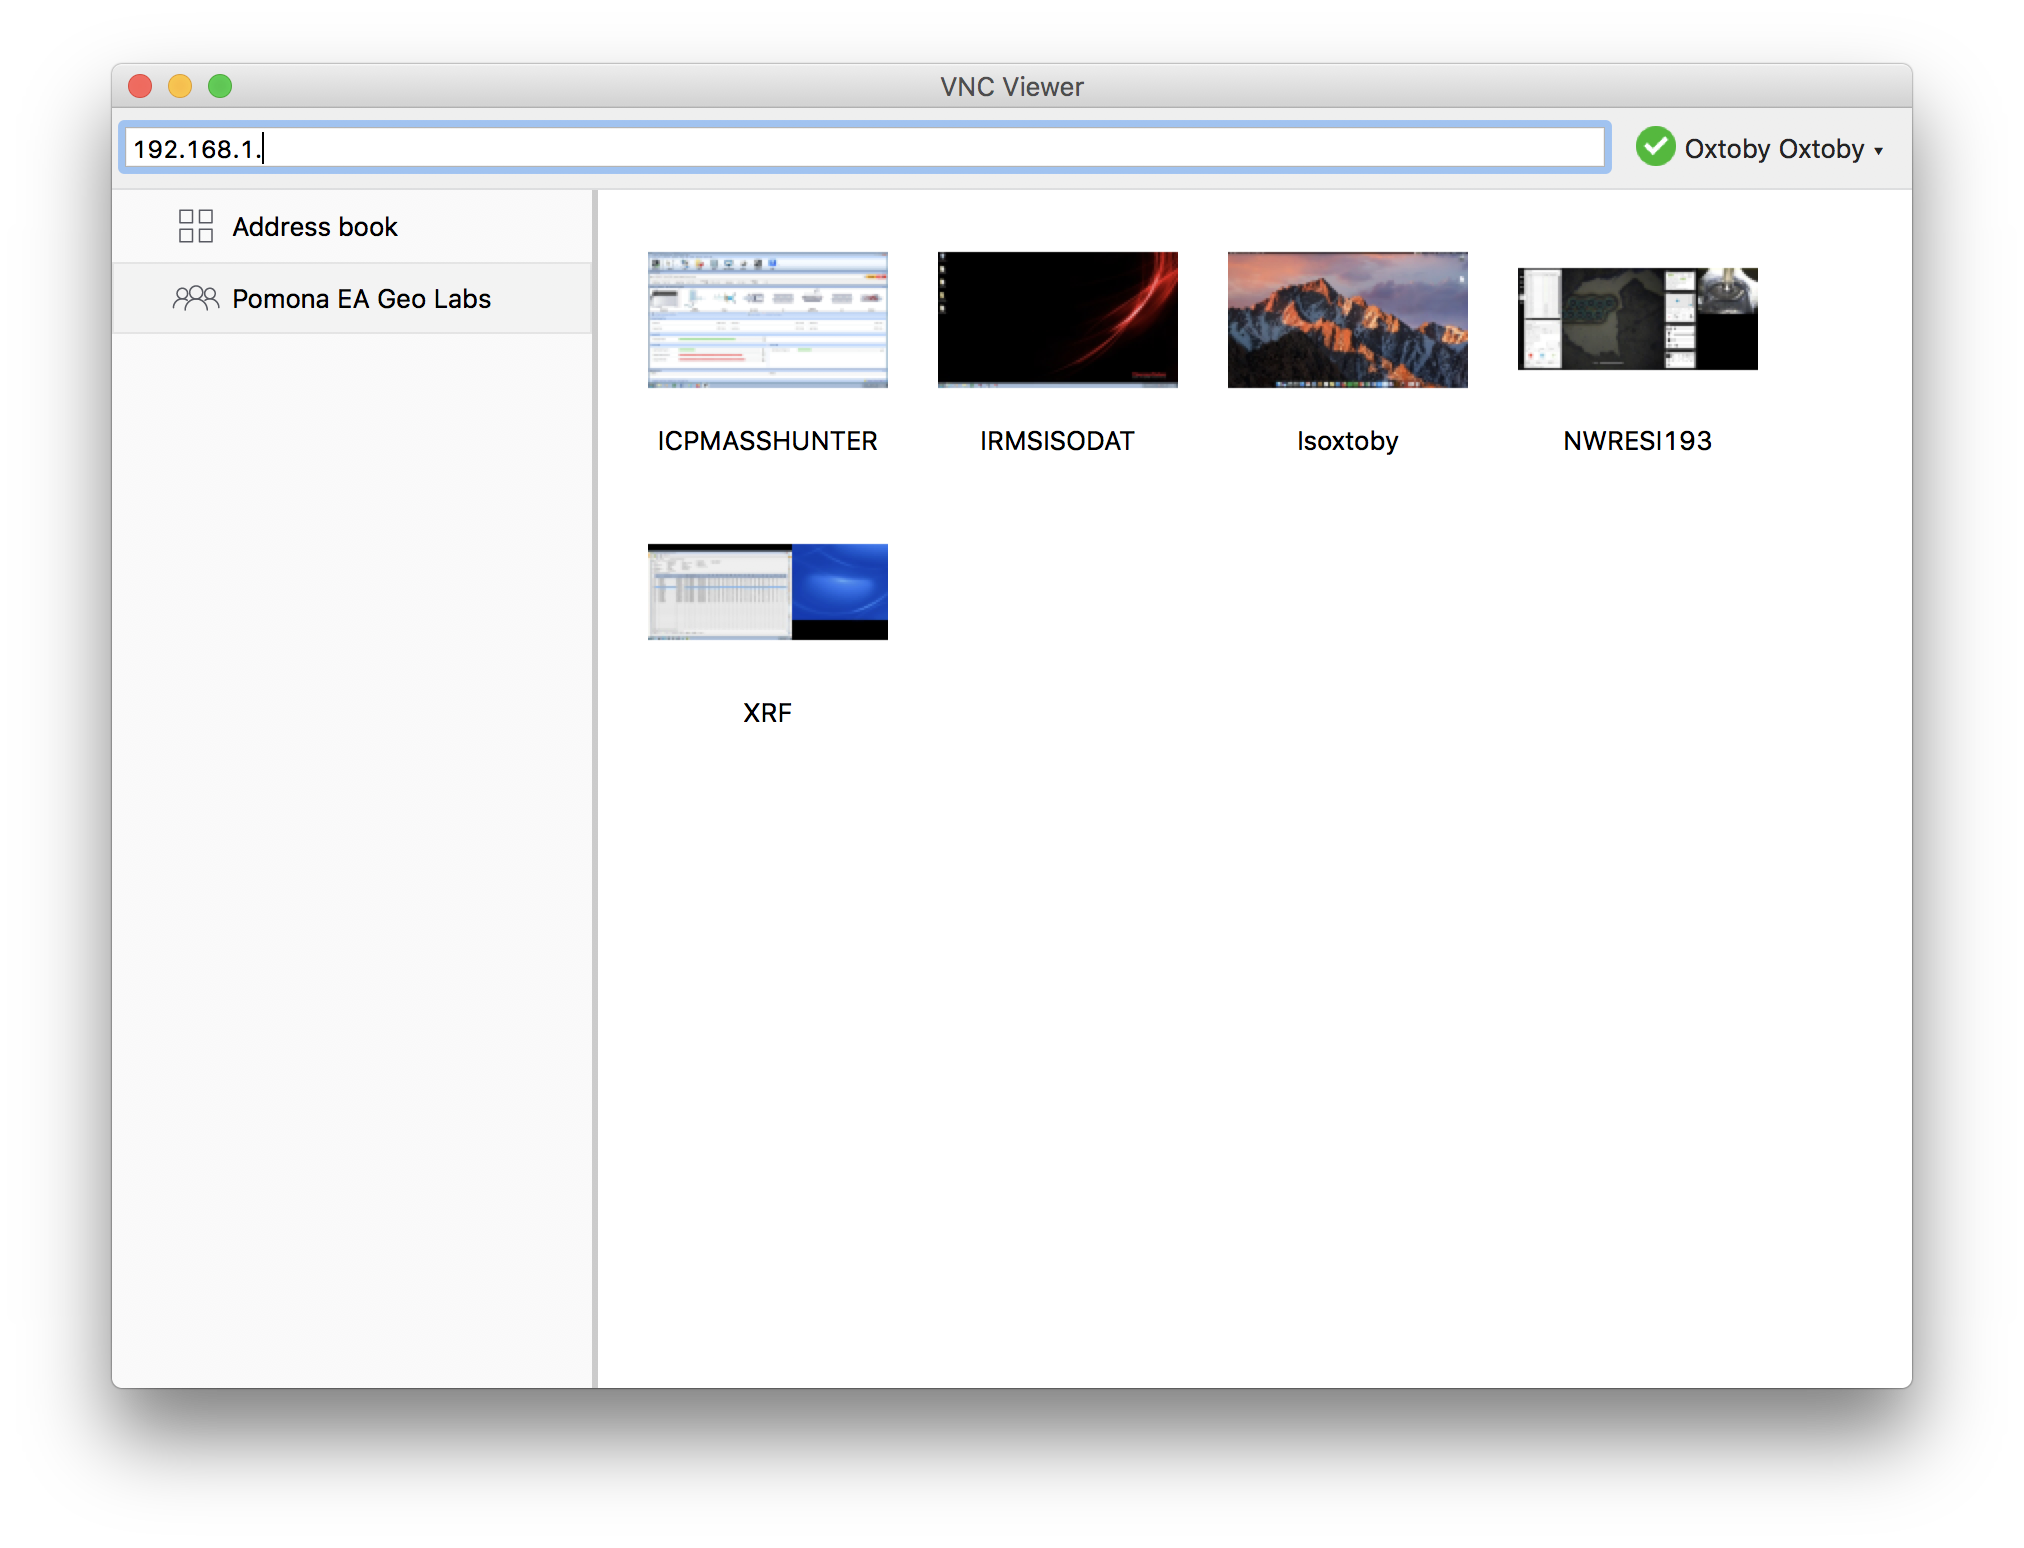
\includegraphics[width=1.00\textwidth]{realvnc}
  \item You will be prompts for the username (pi) and the password -- These are your pi's username and password. Remember changing your password will be a good idea a some point.
  \item Wait a minute and you should eventually see the desktop of the Pi. You can can browse and manipulate with your mouse etc.
\end{enumerate}

\section{Finishing Up}

You Pi should be configured now! When the Pi does get turned off and turned back on, it should boot and connect to your WiFi and allow you to SSH into it. Now, we still need to close the Pi's configuration utility and shut down the Pi.

\begin{enumerate}
  \item While still in the raspi-config utility, navigate down as far as it lets you \textbf{(About raspi-config)}.
  \newline
  \newline
  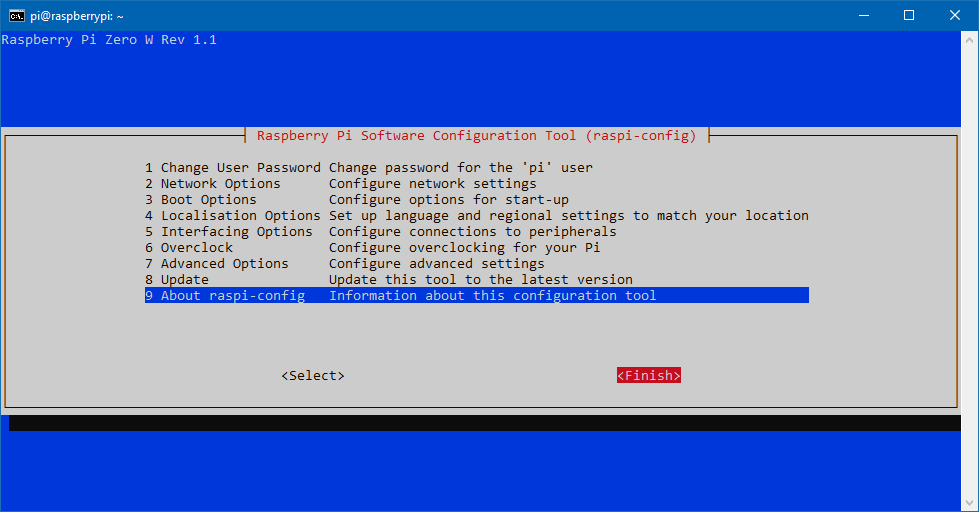
\includegraphics[width=1.00\textwidth]{rcfinish}
  \item You will have to press the right arrow key to get down to \textbf{``FINISH''}. Tricky and a little unintuitive, I know...
  \item Select \textbf{FINISH} and it should exit the utility back to the CLI.
  \item Next, run this last command in the CLI to shutdown the Pi:
  \begin{lstlisting}
  sudo shutdown -h now
  \end{lstlisting}
  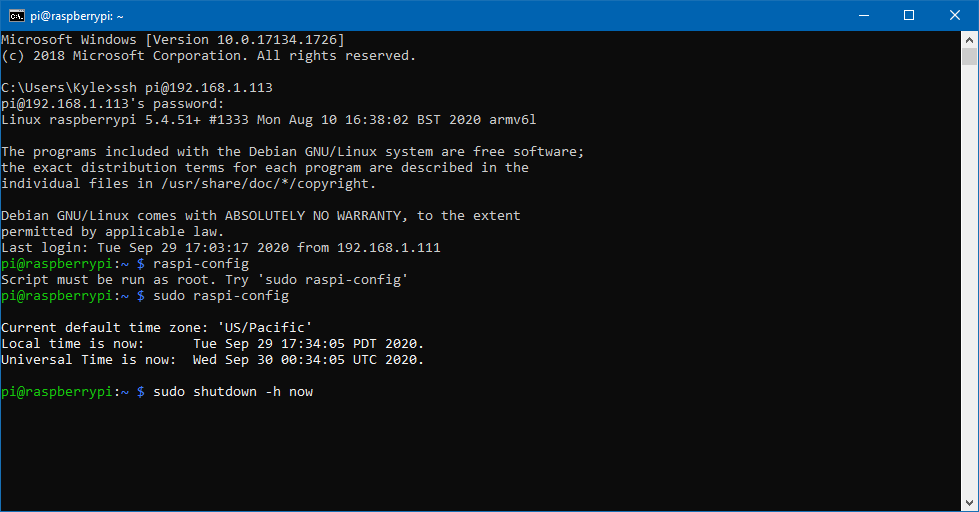
\includegraphics[width=1.00\textwidth]{sudoshutdown}
  \item Soon the Pi will shutdown and you'll get a message in your Command Prompt/Terminal something along the lines that the connection was closed or lost. 
  \newline
  \newline
  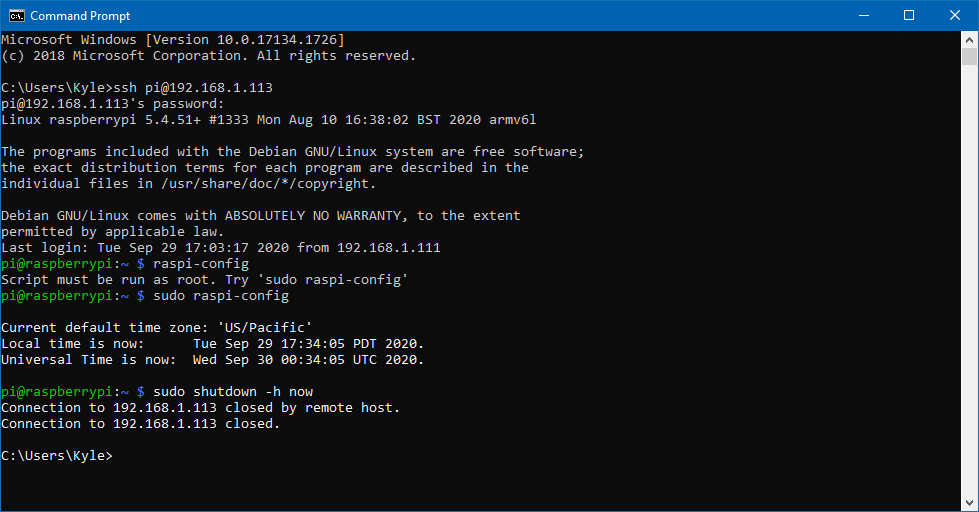
\includegraphics[width=1.00\textwidth]{sshshutdown}
  \item Flip the switch on the power supply to the Pi to make sure power is not going to the Pi.
\end{enumerate}

\textbf{CONGRATULATIONS}! You done configuring the Pi. \textit{Whew}...

\end{document}
